\documentclass[11pt,letterpaper]{article}
\input{headings}
\newcommand \recipeName {Pork Knuckle}
\newcommand \fileName {PorkKnuckle}
\chead{\recipeName}

\begin{document}
\input{title}

This recipe I first saw in my mother's (Dioraci Rambo Urtassum) cookbook {\it Del\'icias, aromas, e vidas}. Like many of my mom's recipe, this one is streamlined and simple, but surprisingly delicious. If you would like a more elaborate recipe, check out \href {TwelveHourPorkShank.html} {Twelve-Hour Pork Shank}.



\begin{description}

\item[Ingredients:]\ \\
	\begin{itemize}
	\item 1 or 2 pork shanks
	\item	salt
	\item 2 Tbs of unflavoured cooking oil
	\item 1 large onion, sliced
	\item 2 cloves of garlic, minced
	\item 1 red pepper in vinegar, without the seeds, minced
	\end{itemize}

\item[Procedure:]\ \\

	\begin{enumerate}
	\item {\bf Seasoning the shanks}
	\begin{itemize}
	\item Rub the pork shanks with salt and with the red pepper.
	\item Let it rest in the fridge for at least two hours, or up to 24 hours.
	\end{itemize}

	\item {\bf Brown the shanks}
	\begin{itemize}
	\item Rub the minced garlic in the shanks.
	\item Pour the oil in a skillet and place over moderate heat until hot.
	\item Lightly brown all sides of the shanks.
	\item Transfer to a pressure cooker.
	\item Add the sliced onion.
	\item Add enough water to cover the shanks (about 3 cups).
	\item Seal the pressure cooker and bring up to pressure in moderate heat.
	\item Cook under pressure for about 30 minutes.
	\item You can either let it cool in the pressure cooker or you can put the pressure cooker under cold  running water, gently lifting the steam valve under the running water.
	\item Test the shanks with a fork to ensure that they are tender. If they are not tender enough, cover the pressure cooker, bring back to pressure and cook for another 10 minutes.
	\item Cook without the lead to reduce the liquid.
	\item Turn off the fire, move the pot to the side.
	\item Remove the shanks to a plate.
	\item Support one side of the pot with something, such as a wooden board, so that it seats tilted. Let stand for about five minutes so that the fat floats to the top.
	\item Taste to correct seasoning if needed.
	\item Serve warm with peeled potatoes cooked separately with only salt.
	\end{itemize}
	\end{enumerate}
\end{description}
\begin{table}
\begin{tabular}{cccc}
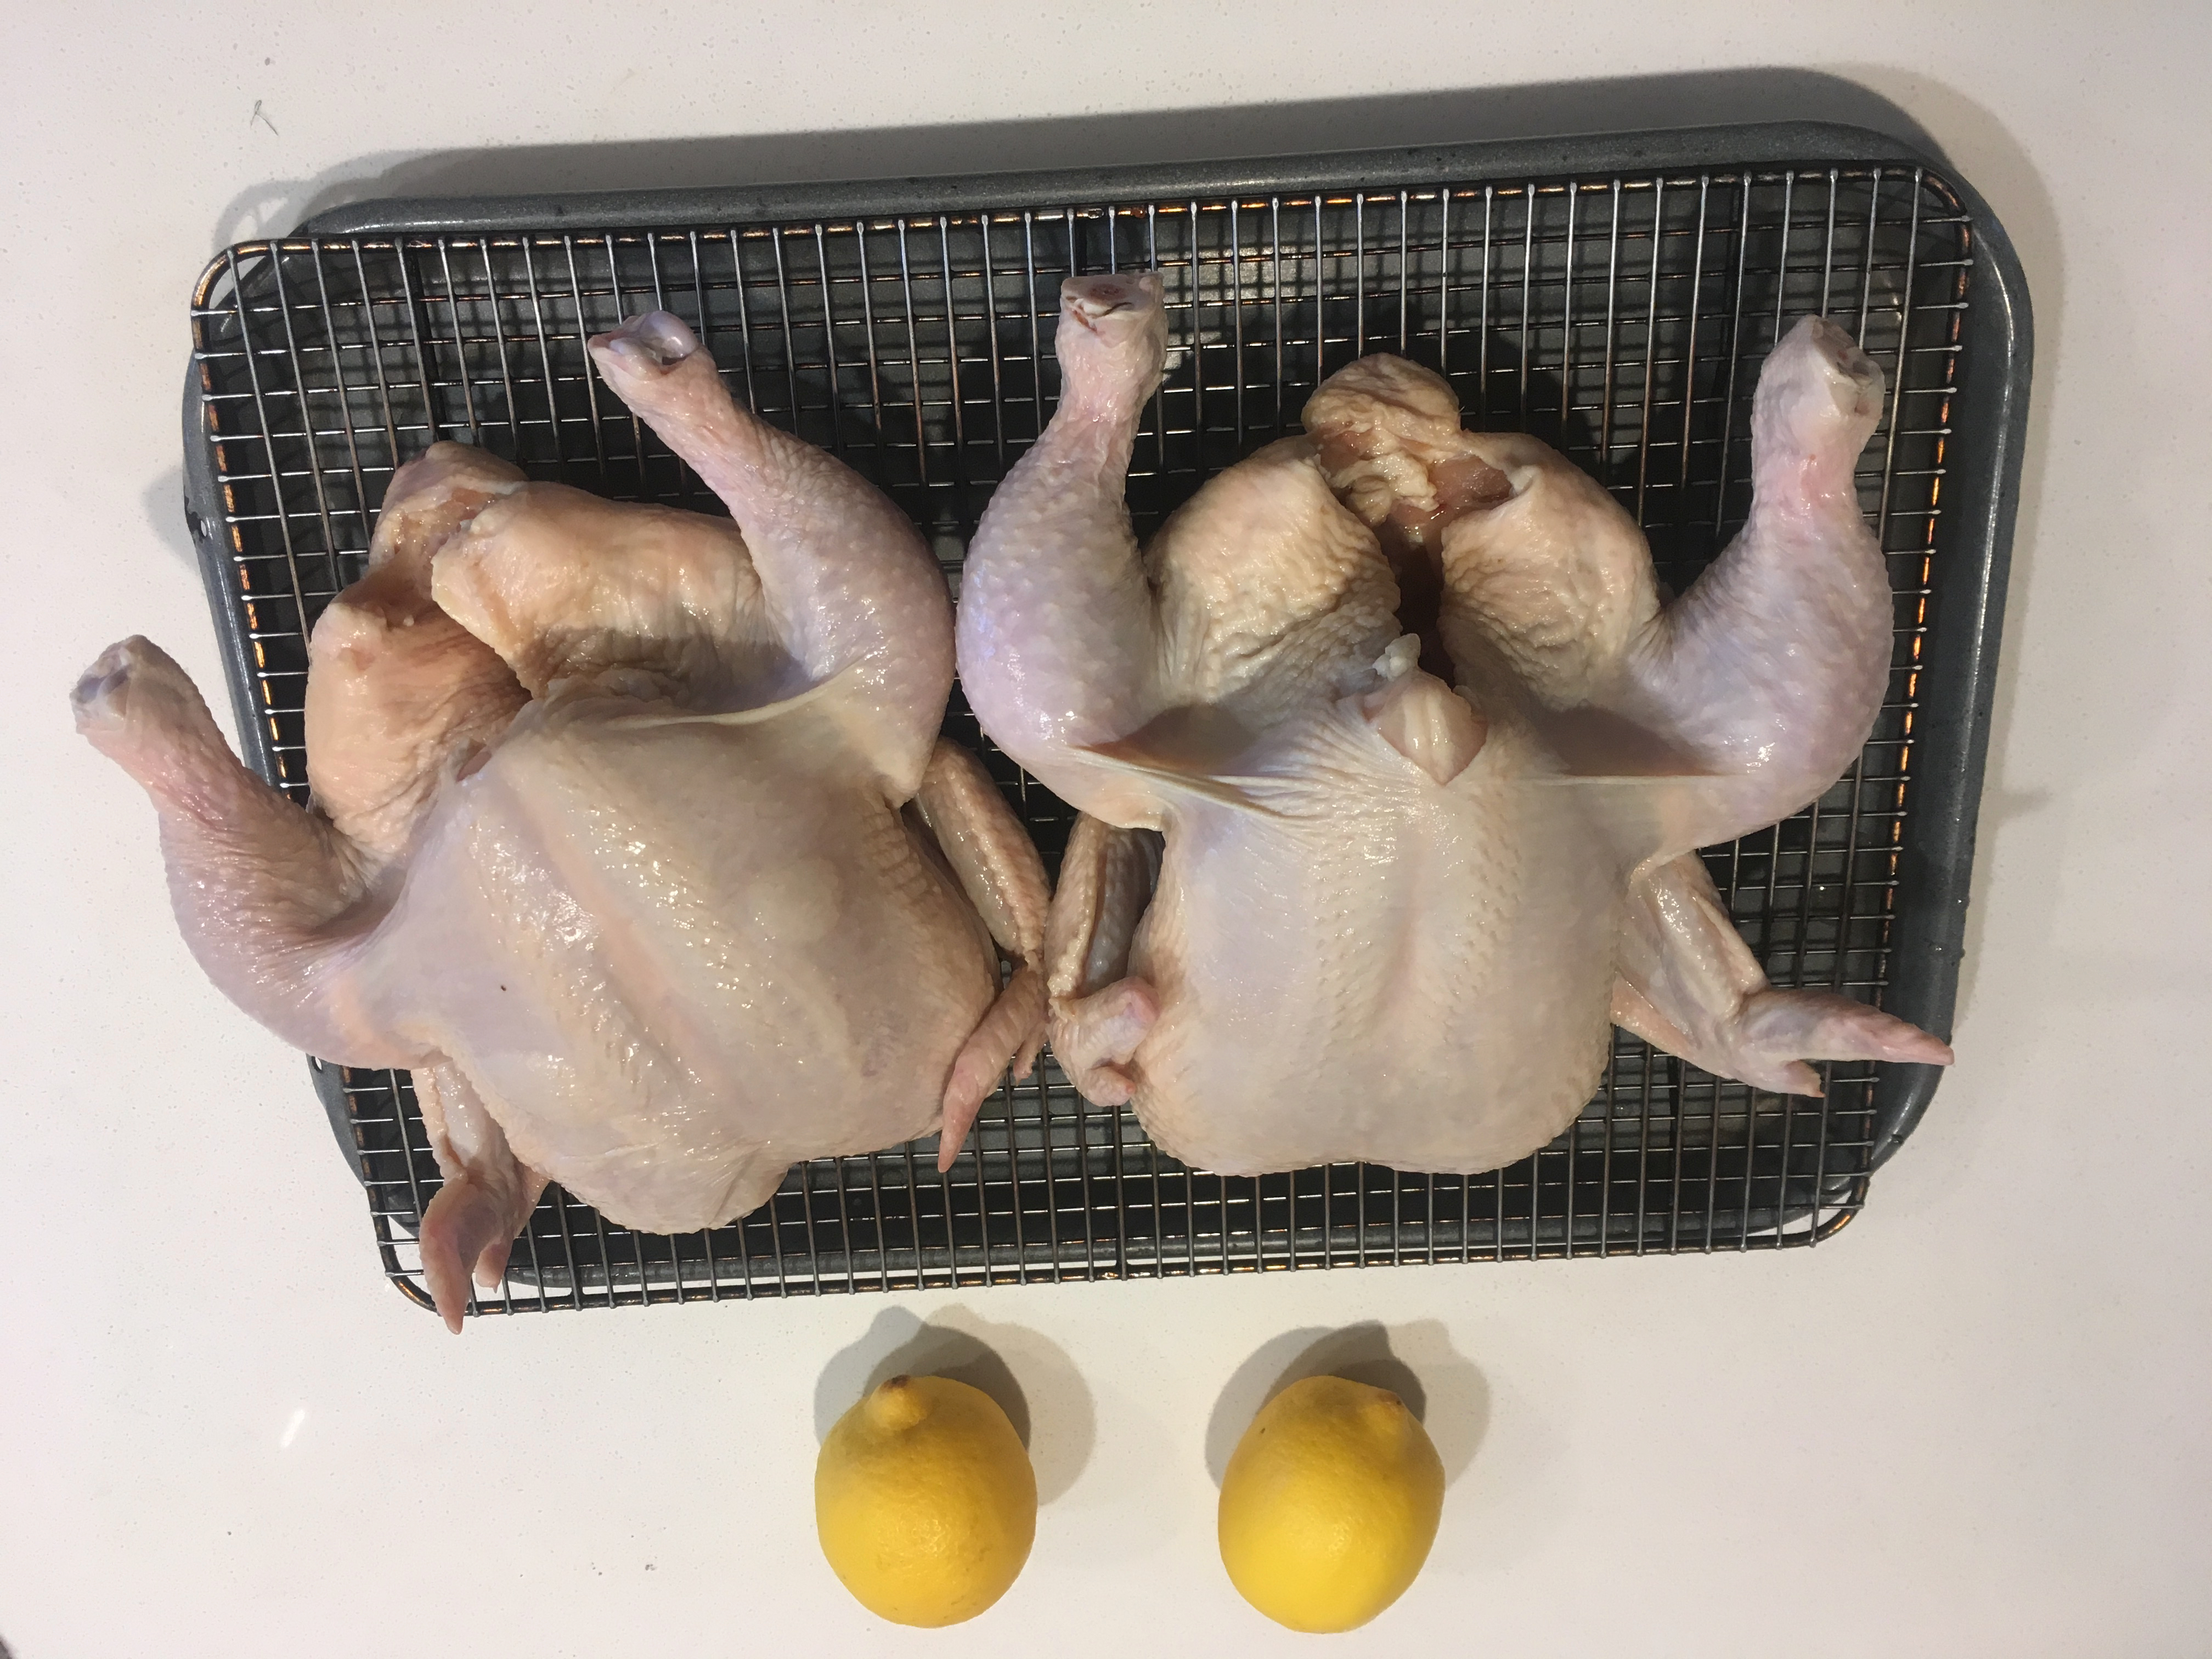
\includegraphics[width=0.25\textwidth]{\imageDir/\fileName/IMG_3197.jpg} &
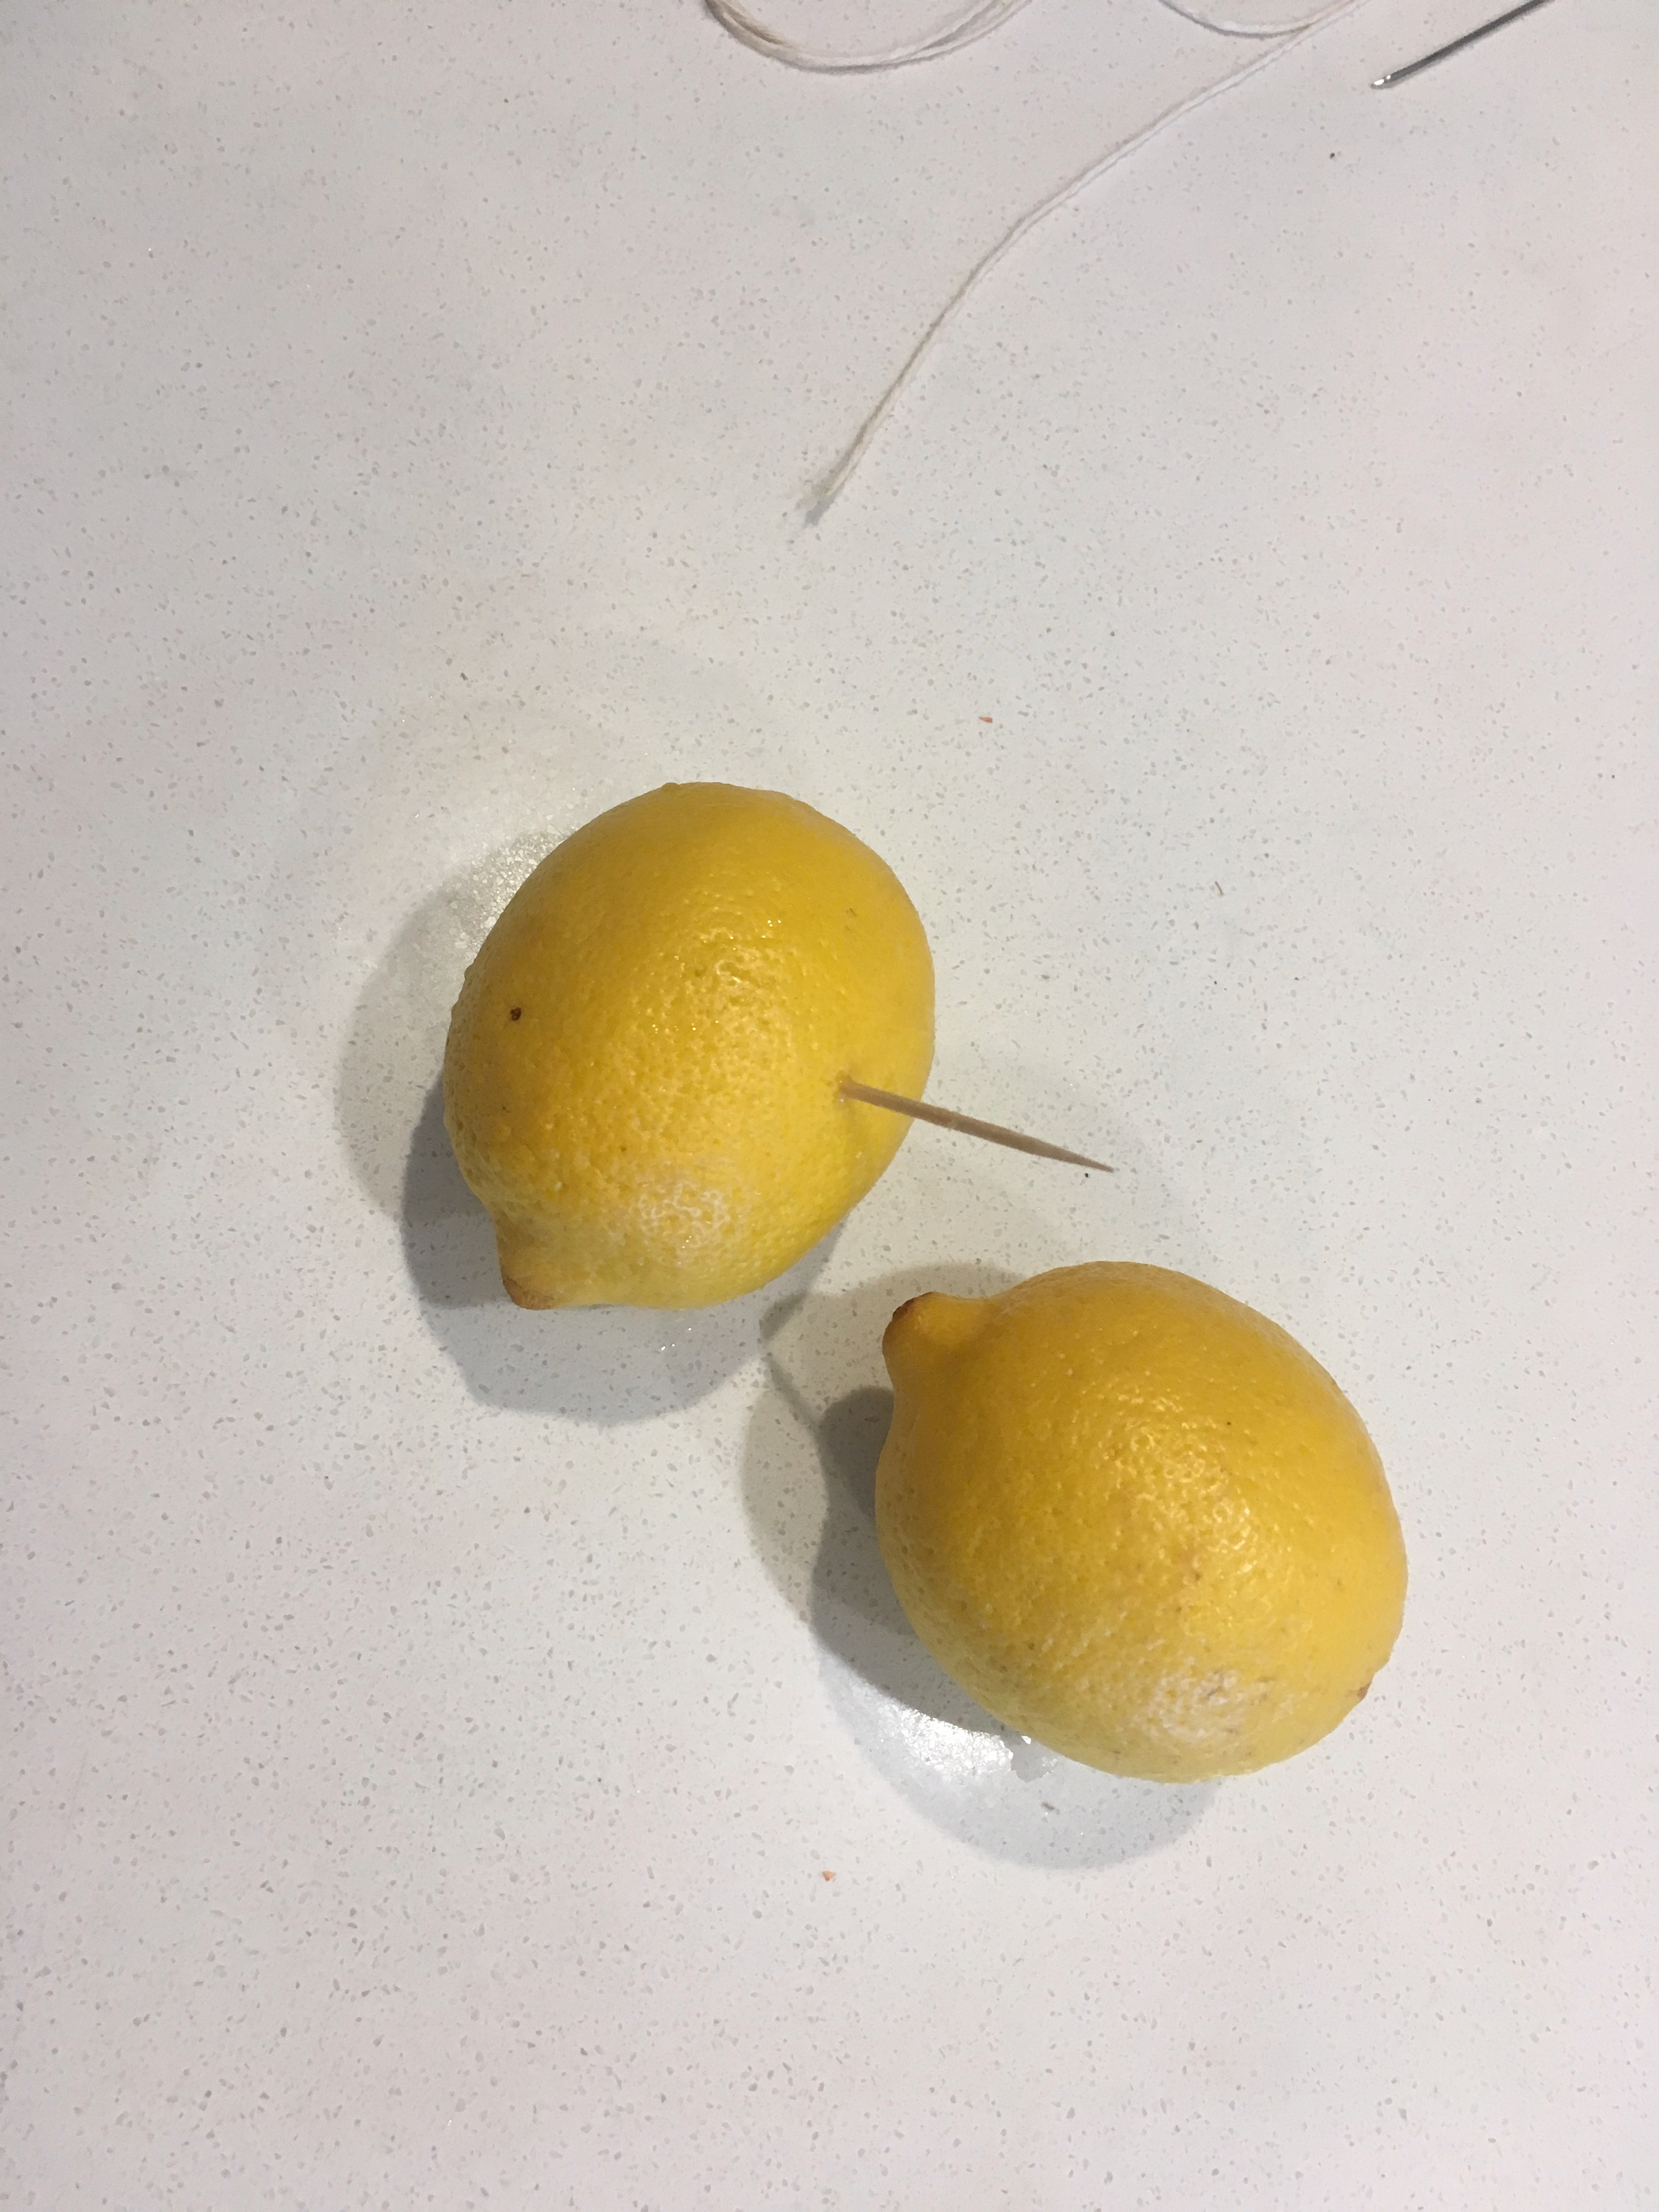
\includegraphics[width=0.25\textwidth]{\imageDir/\fileName/IMG_3212.jpg} &
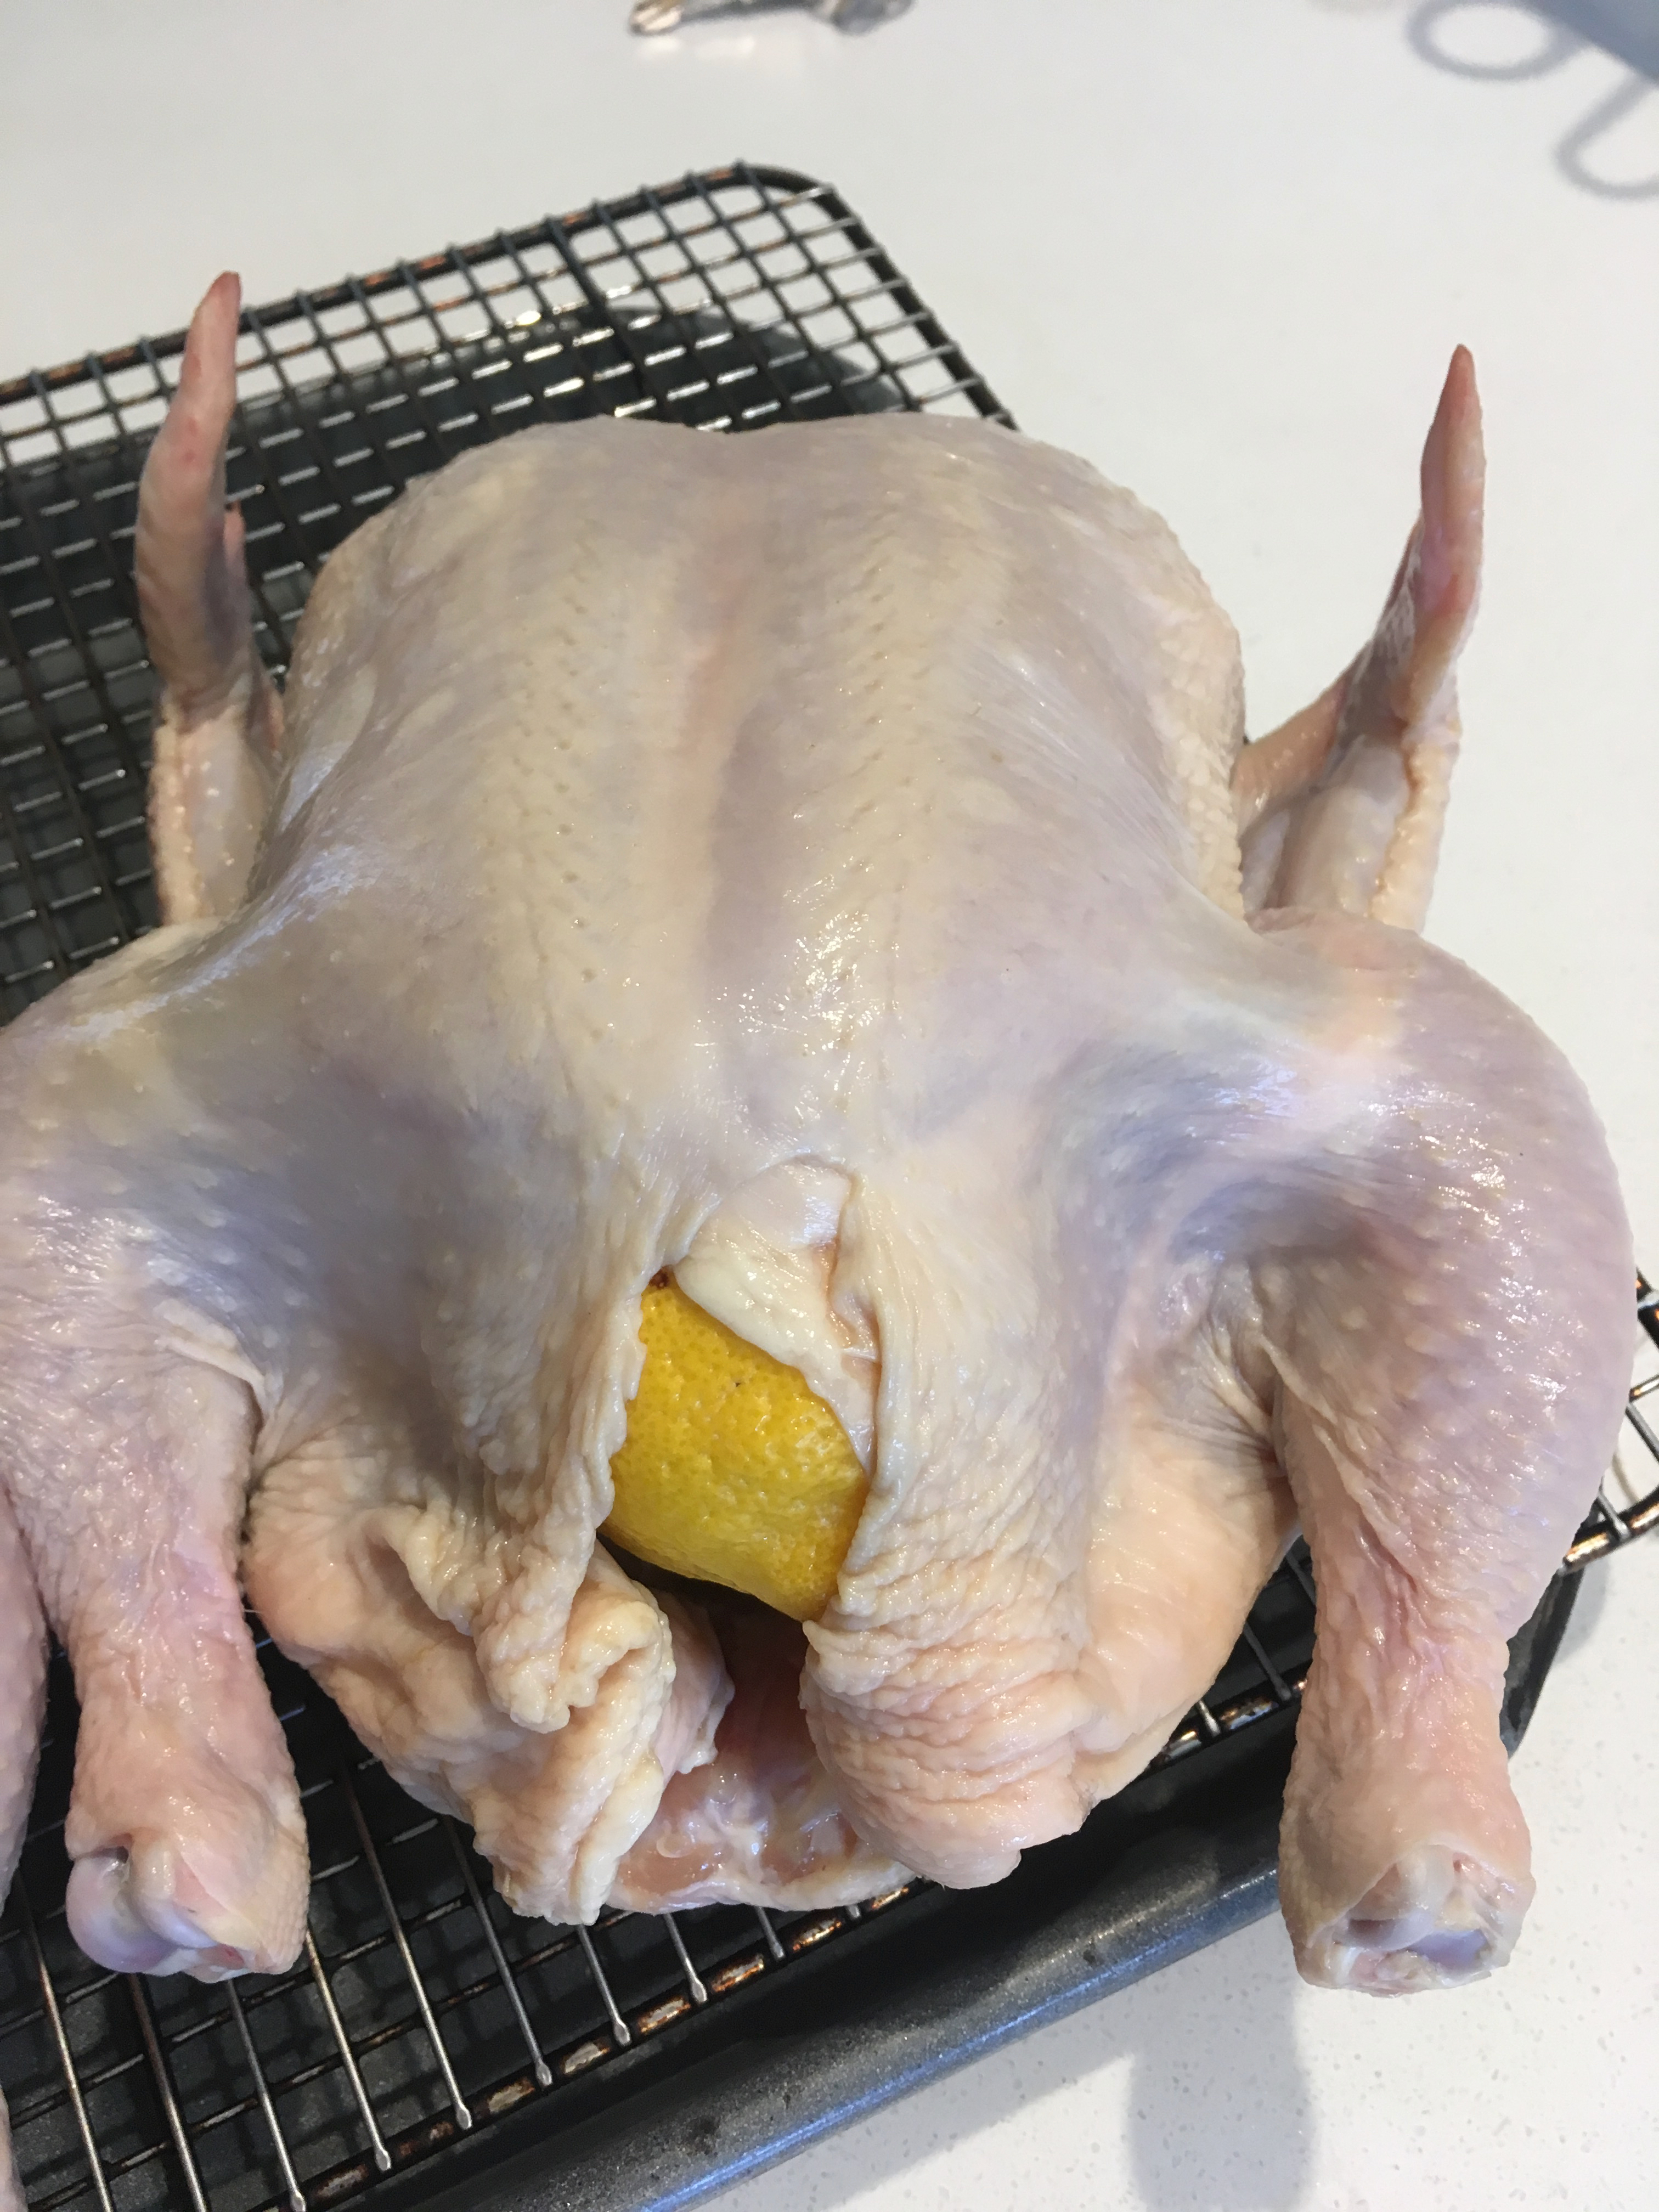
\includegraphics[width=0.25\textwidth]{\imageDir/\fileName/IMG_3213.jpg} \\
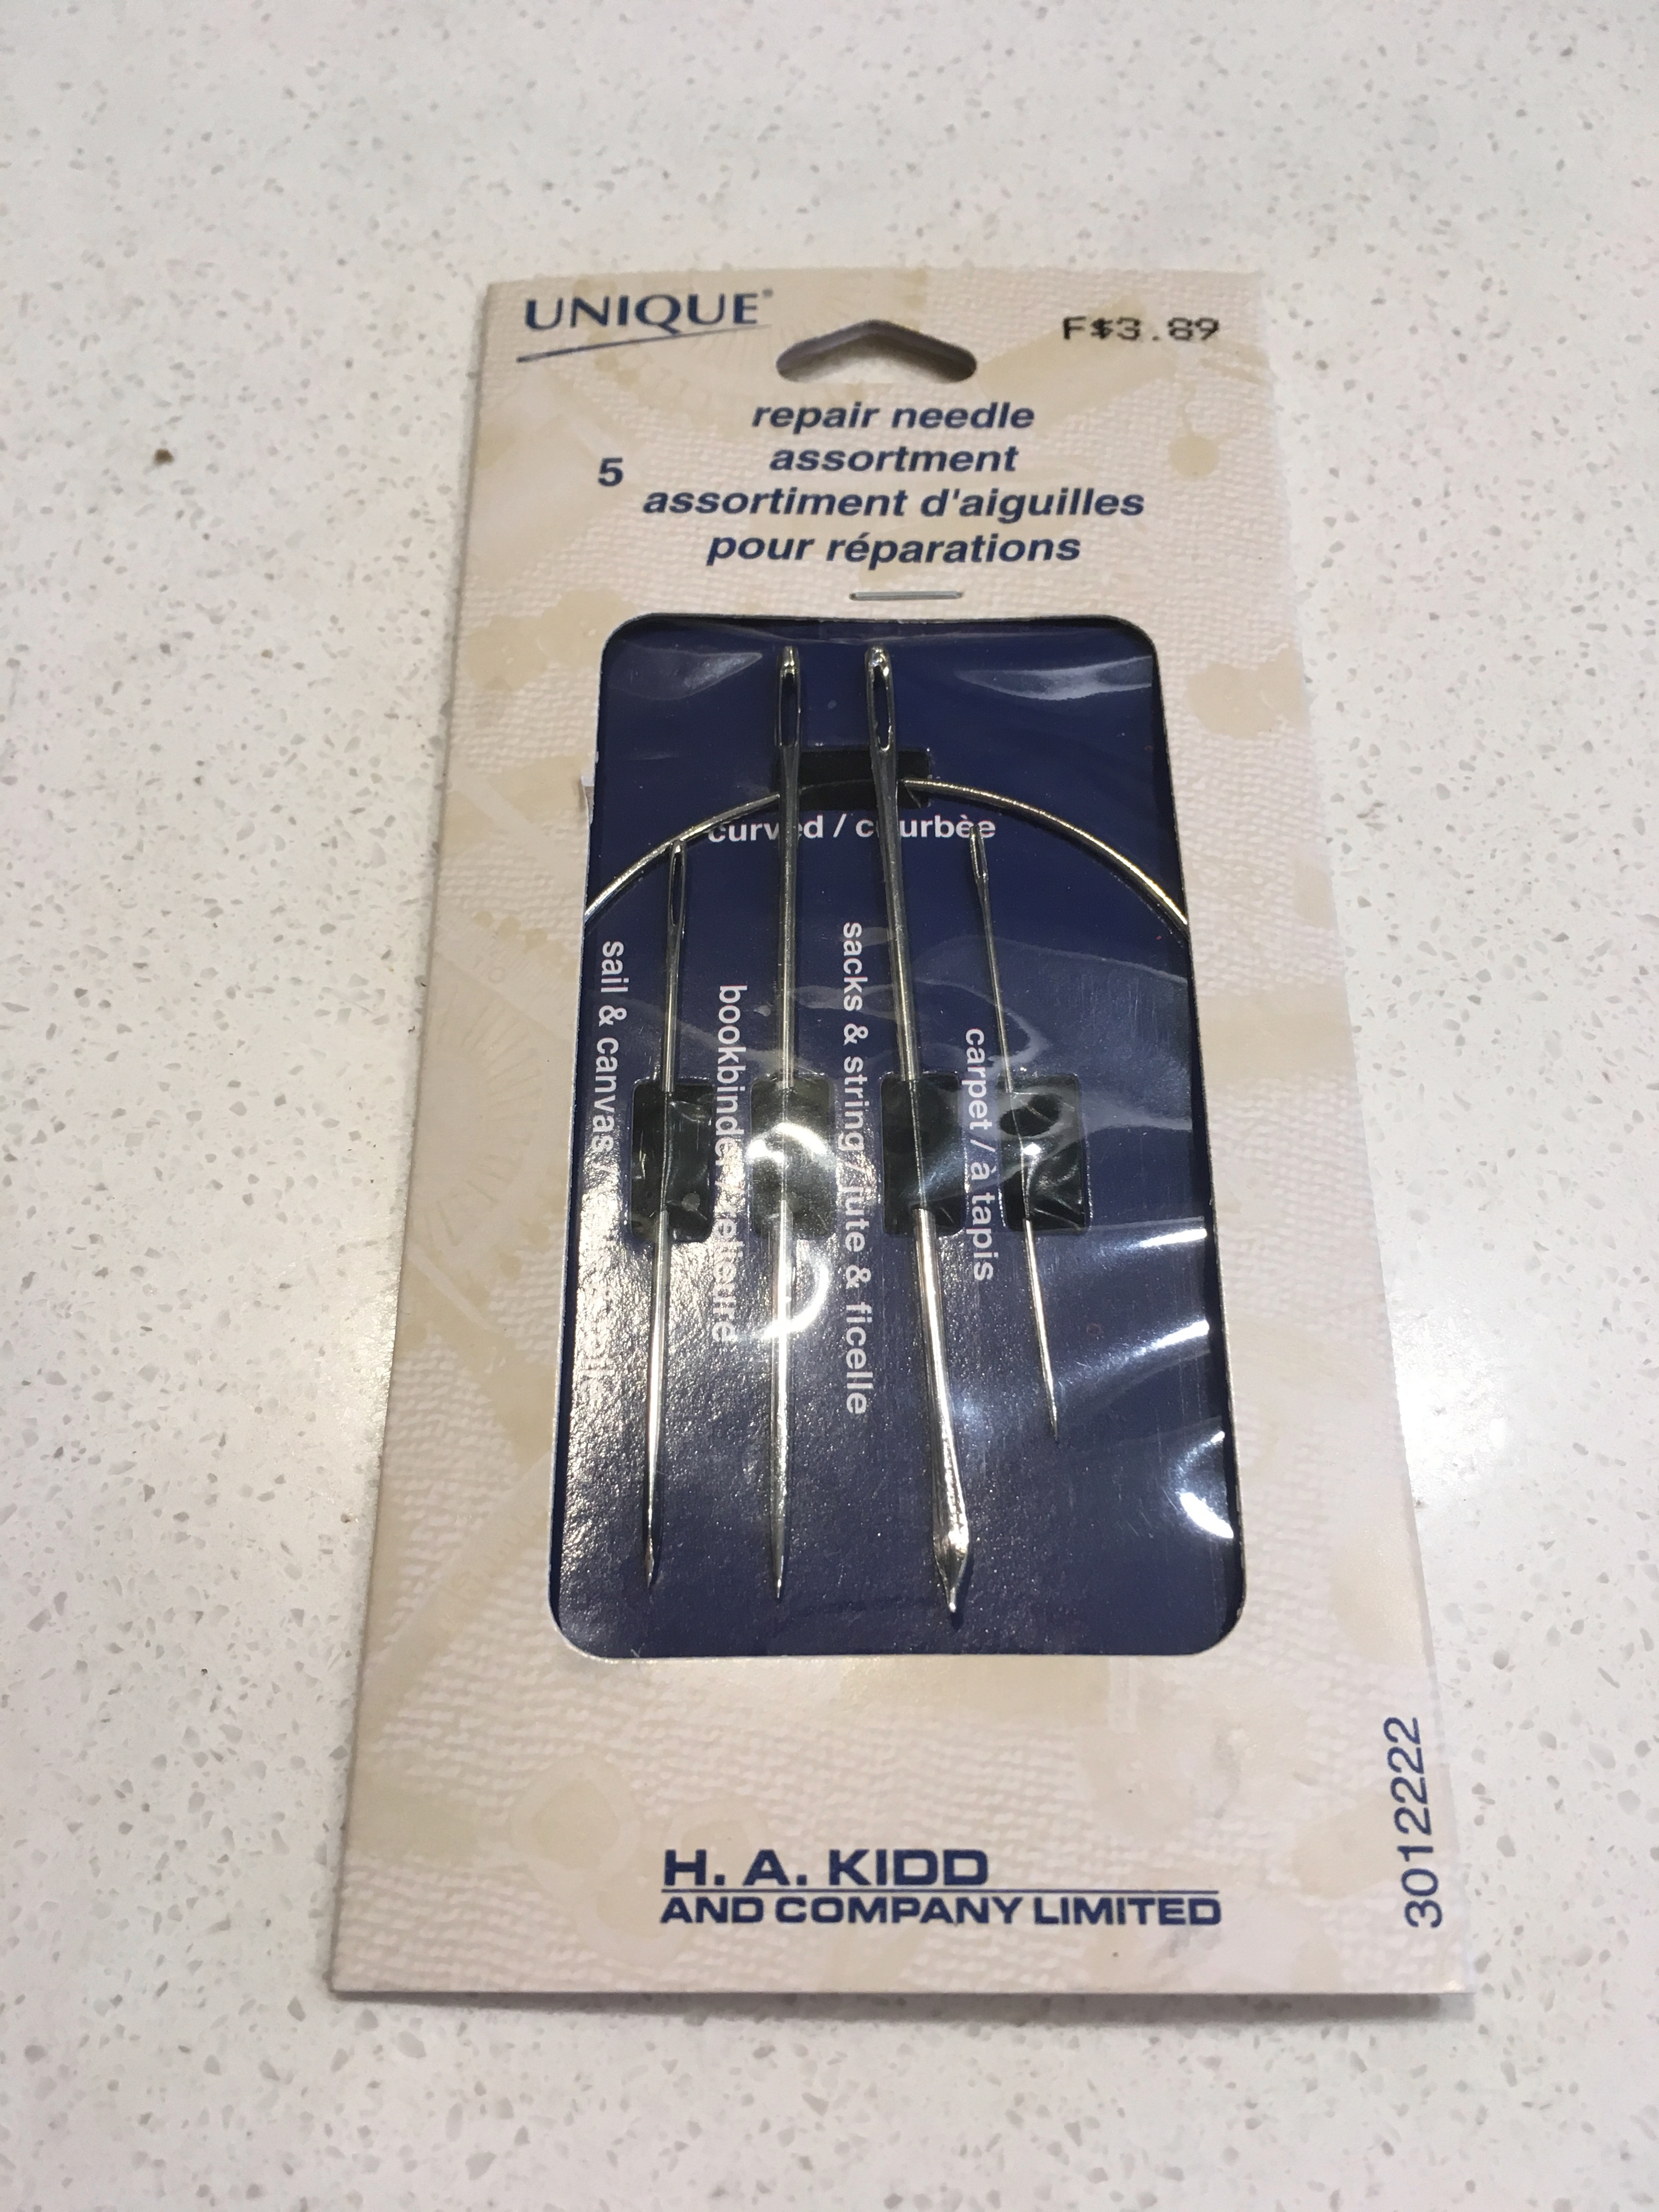
\includegraphics[width=0.25\textwidth]{\imageDir/\fileName/IMG_3206.jpg} &
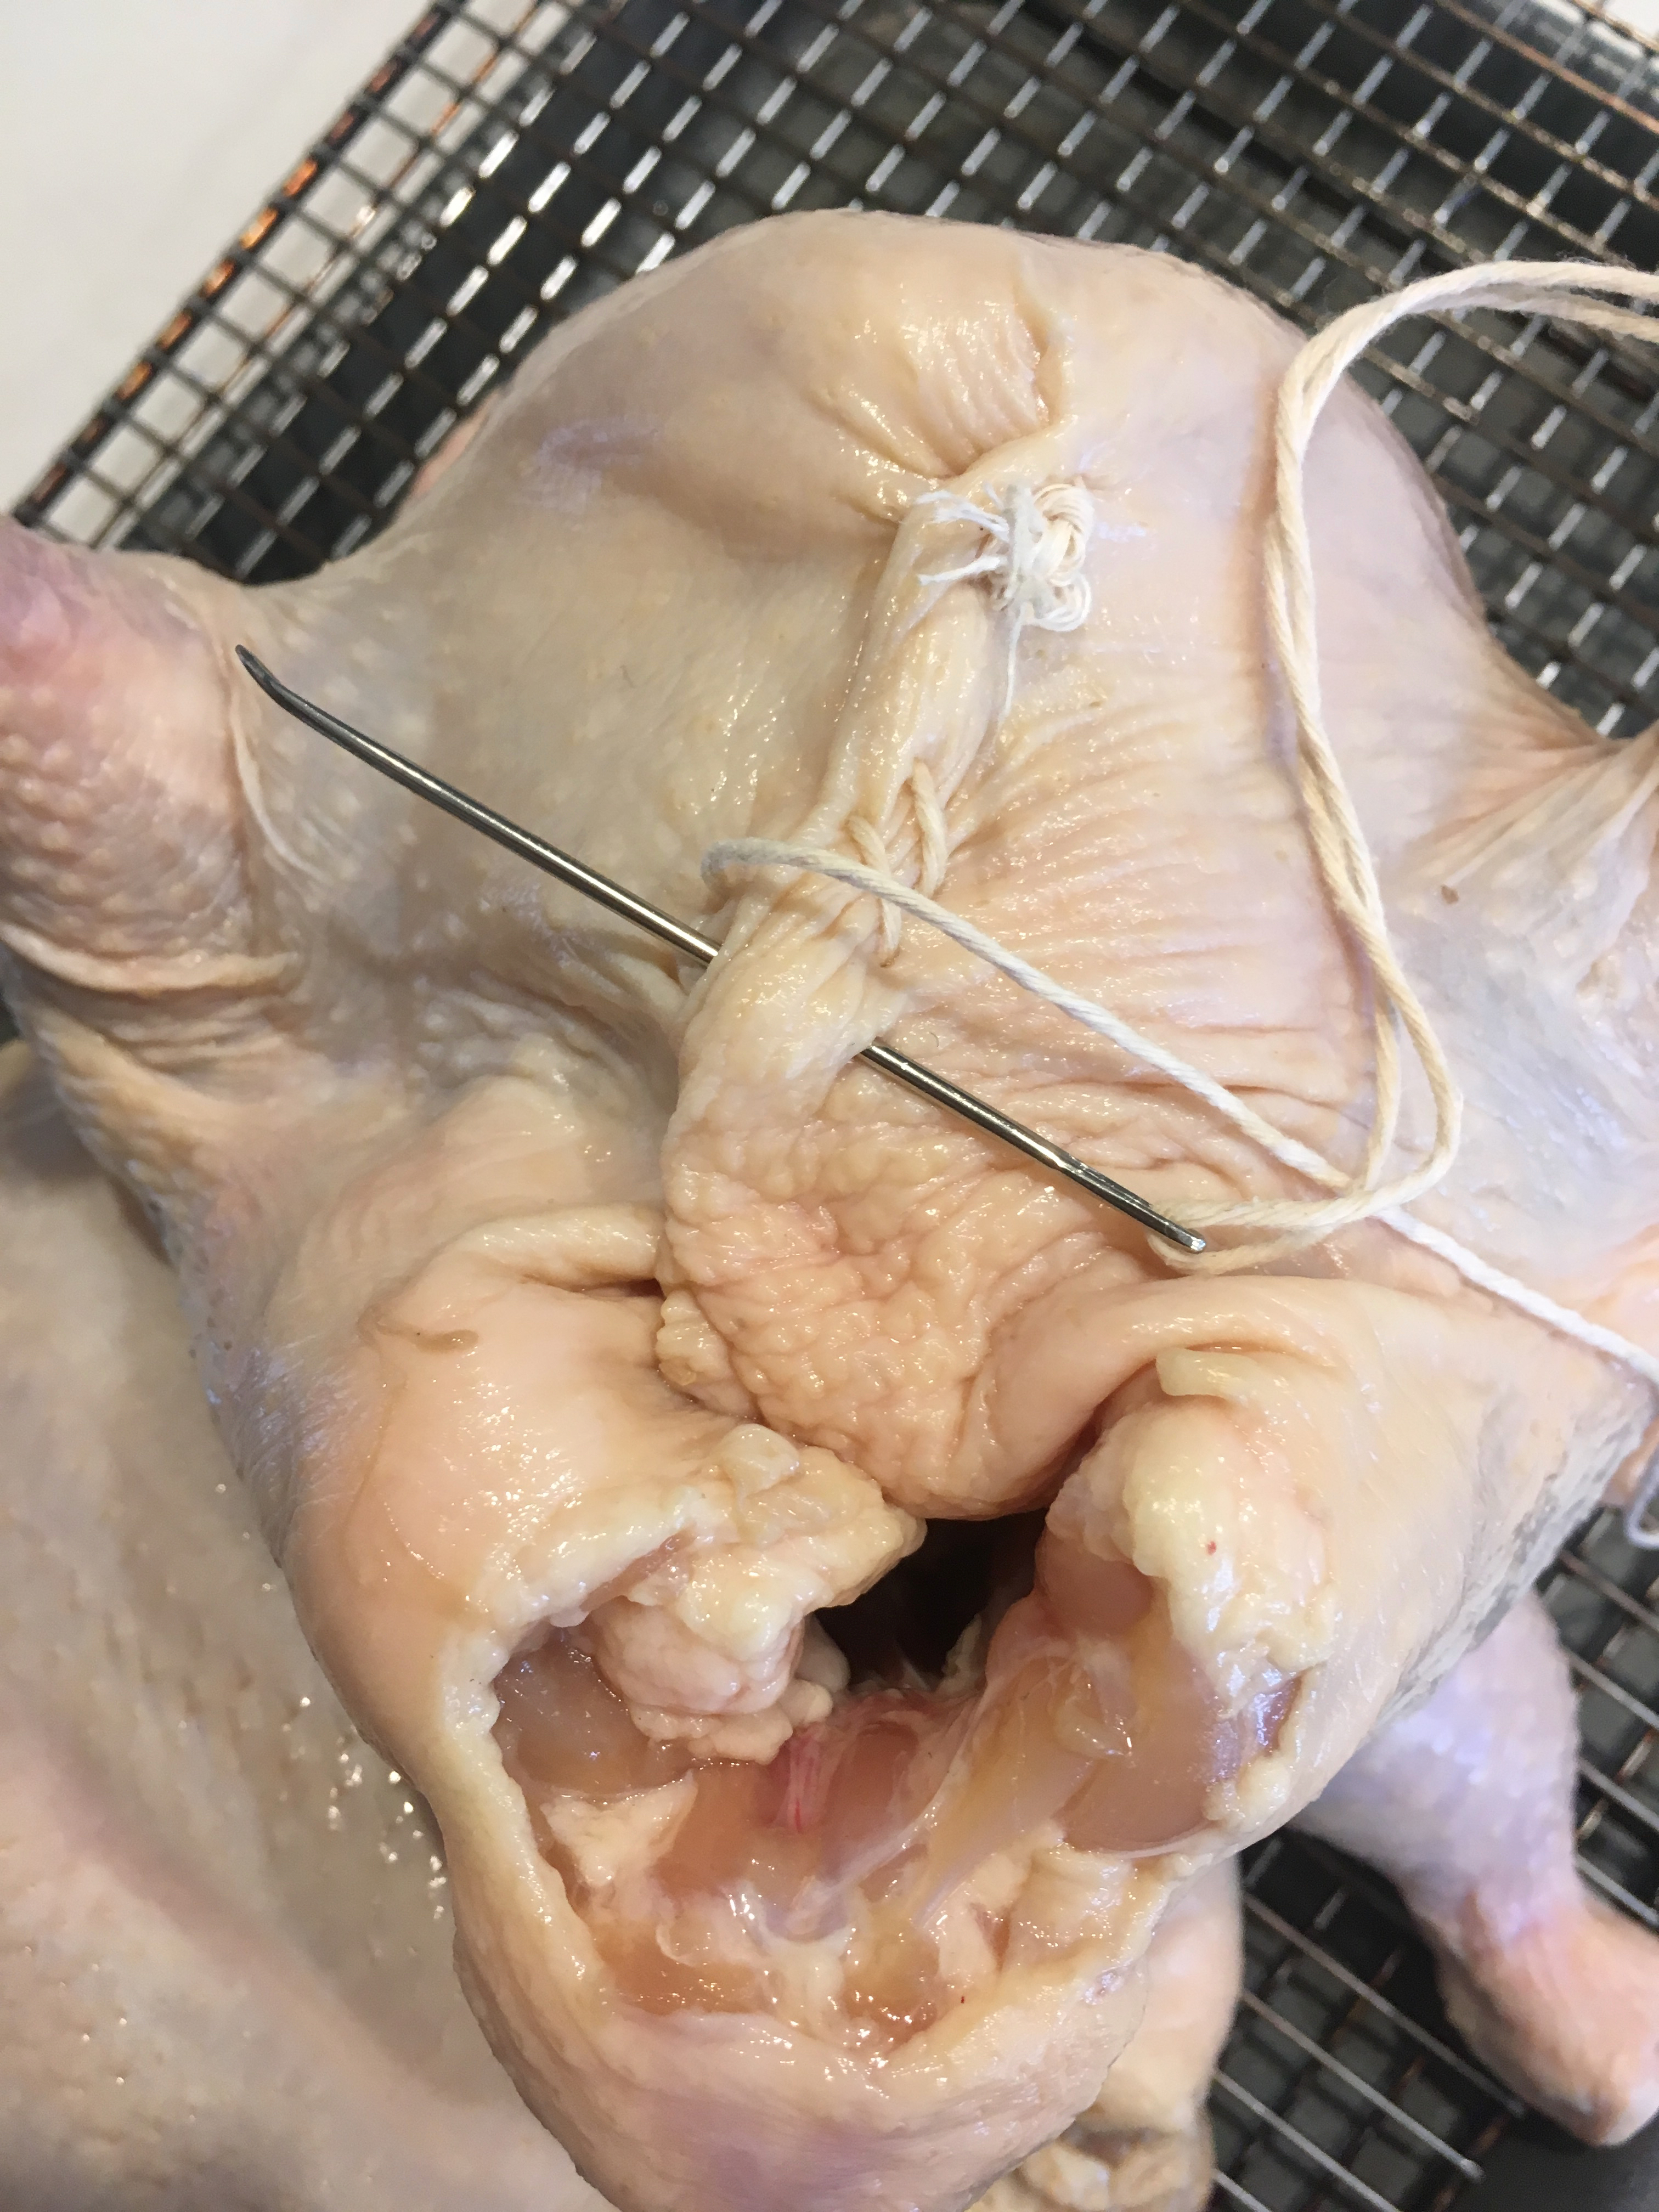
\includegraphics[width=0.25\textwidth]{\imageDir/\fileName/IMG_3214.jpg} &
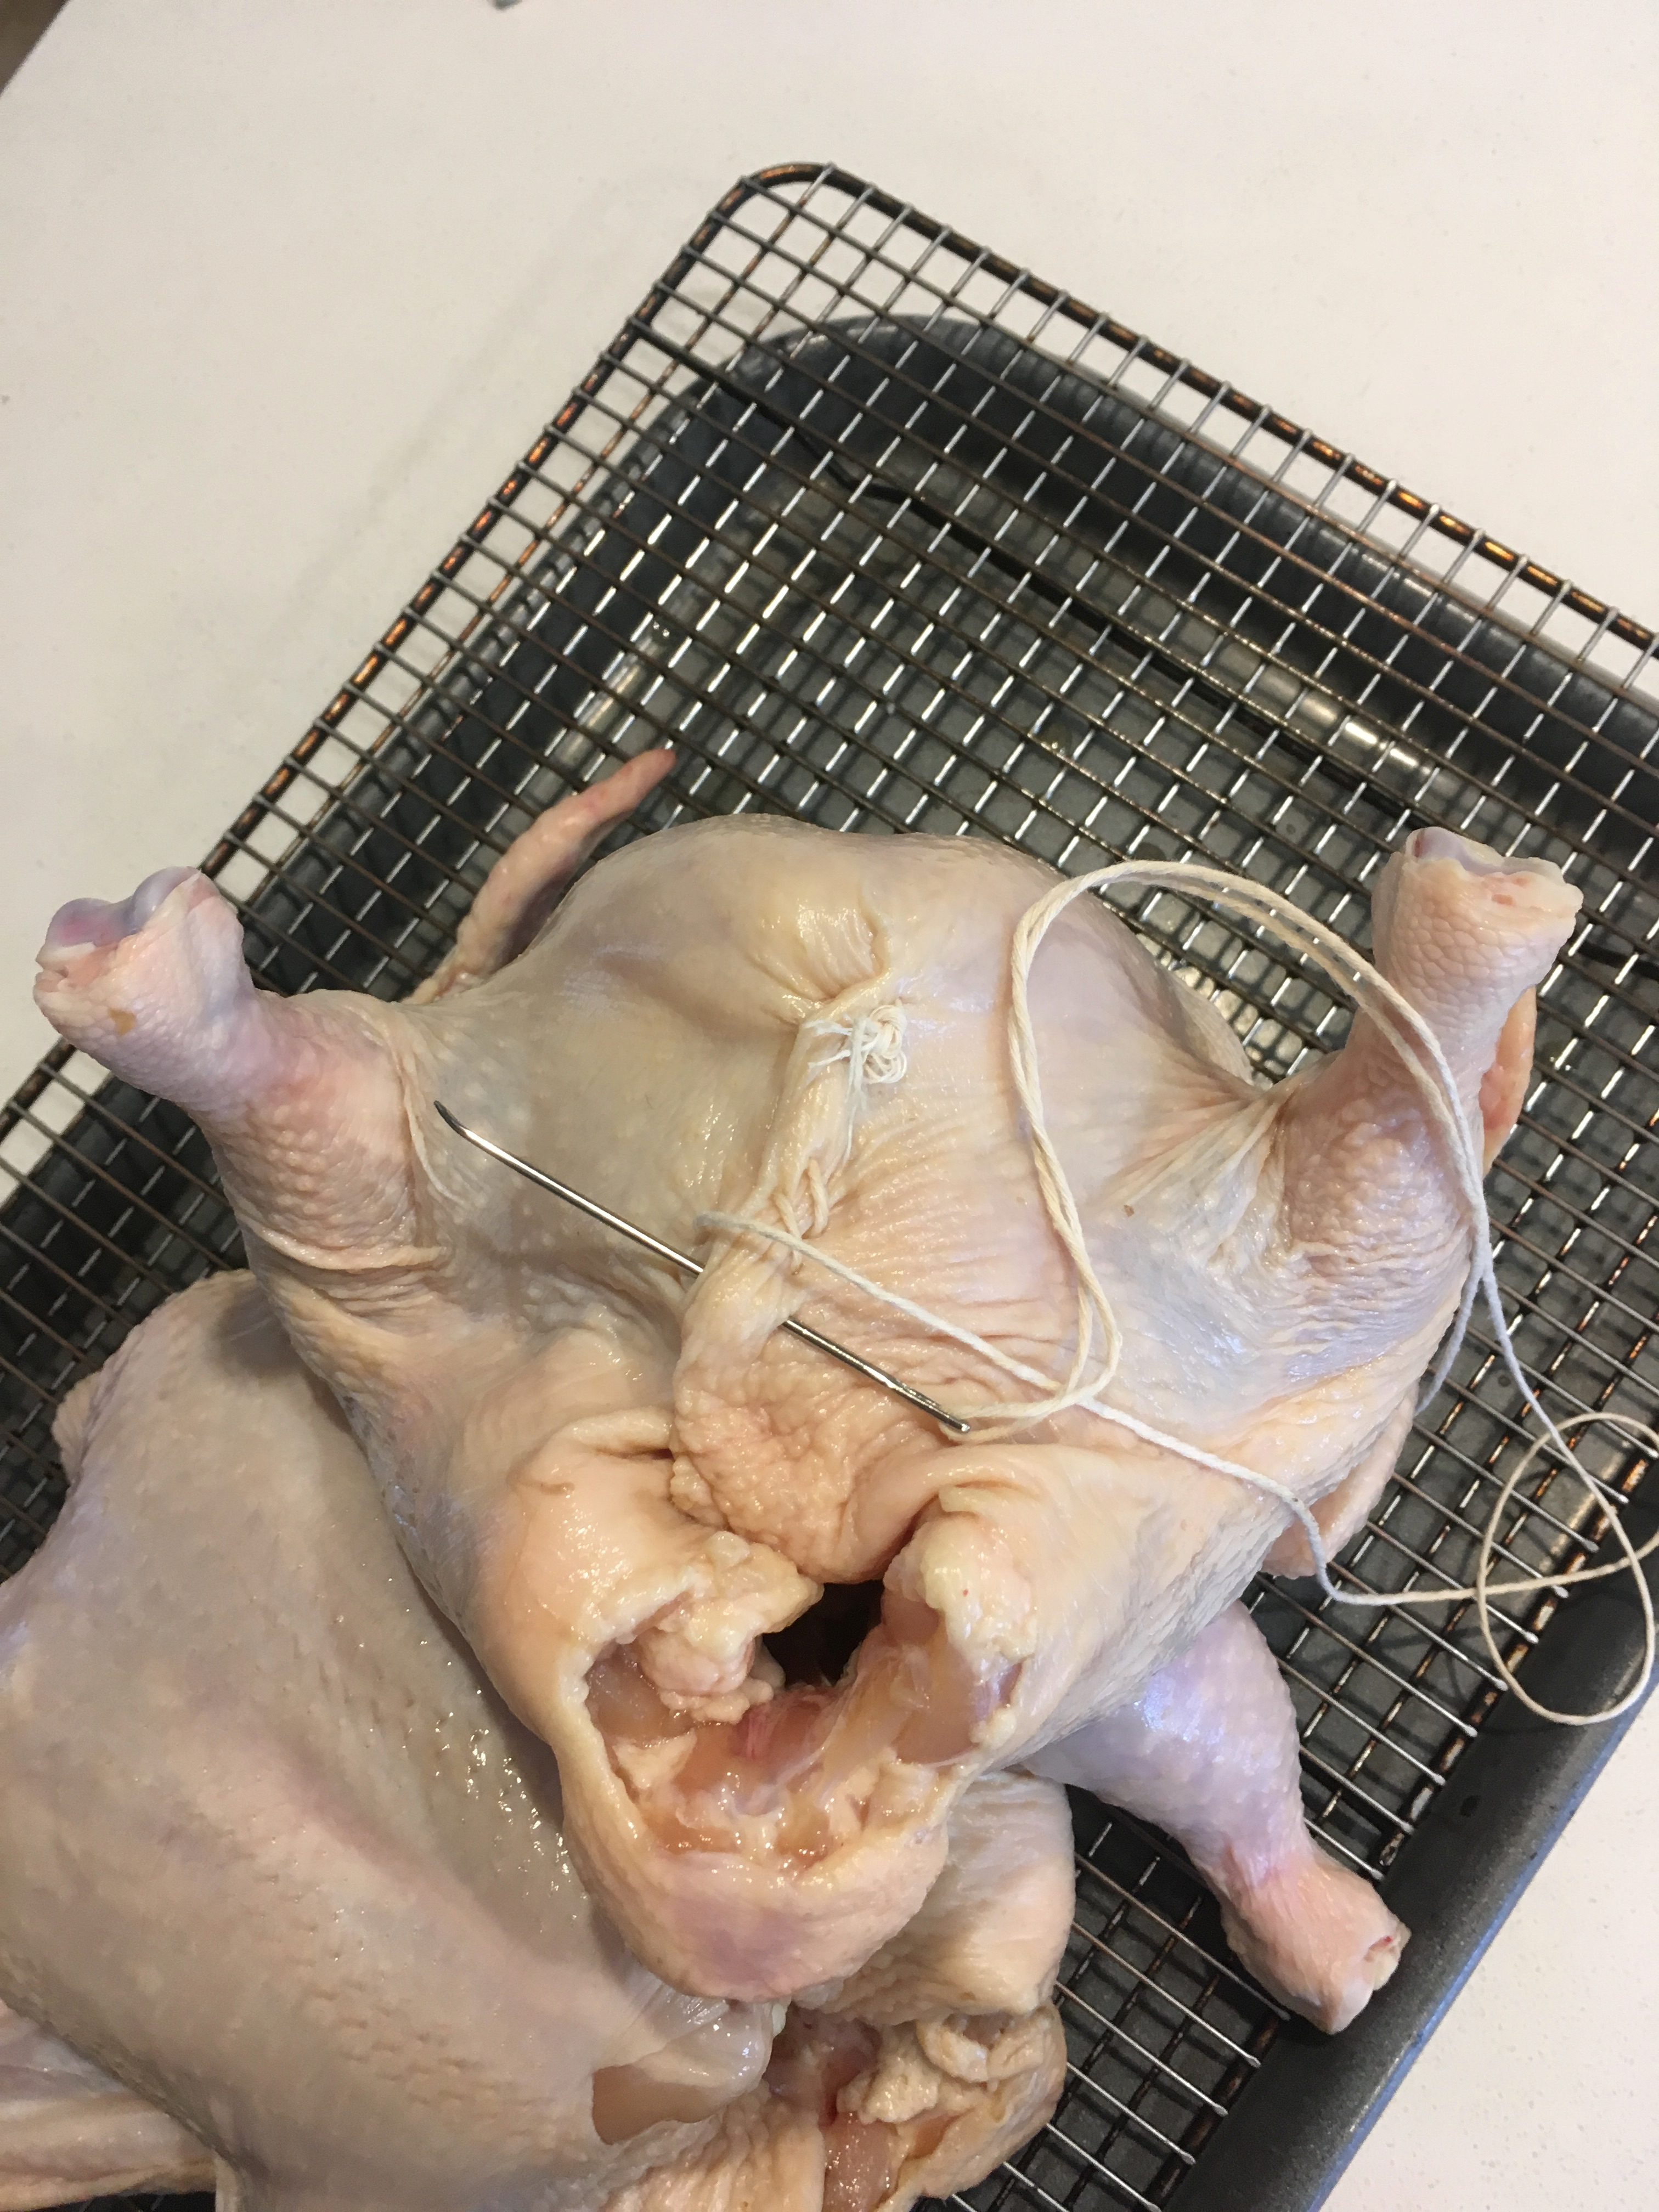
\includegraphics[width=0.25\textwidth]{\imageDir/\fileName/IMG_3216.jpg} \\
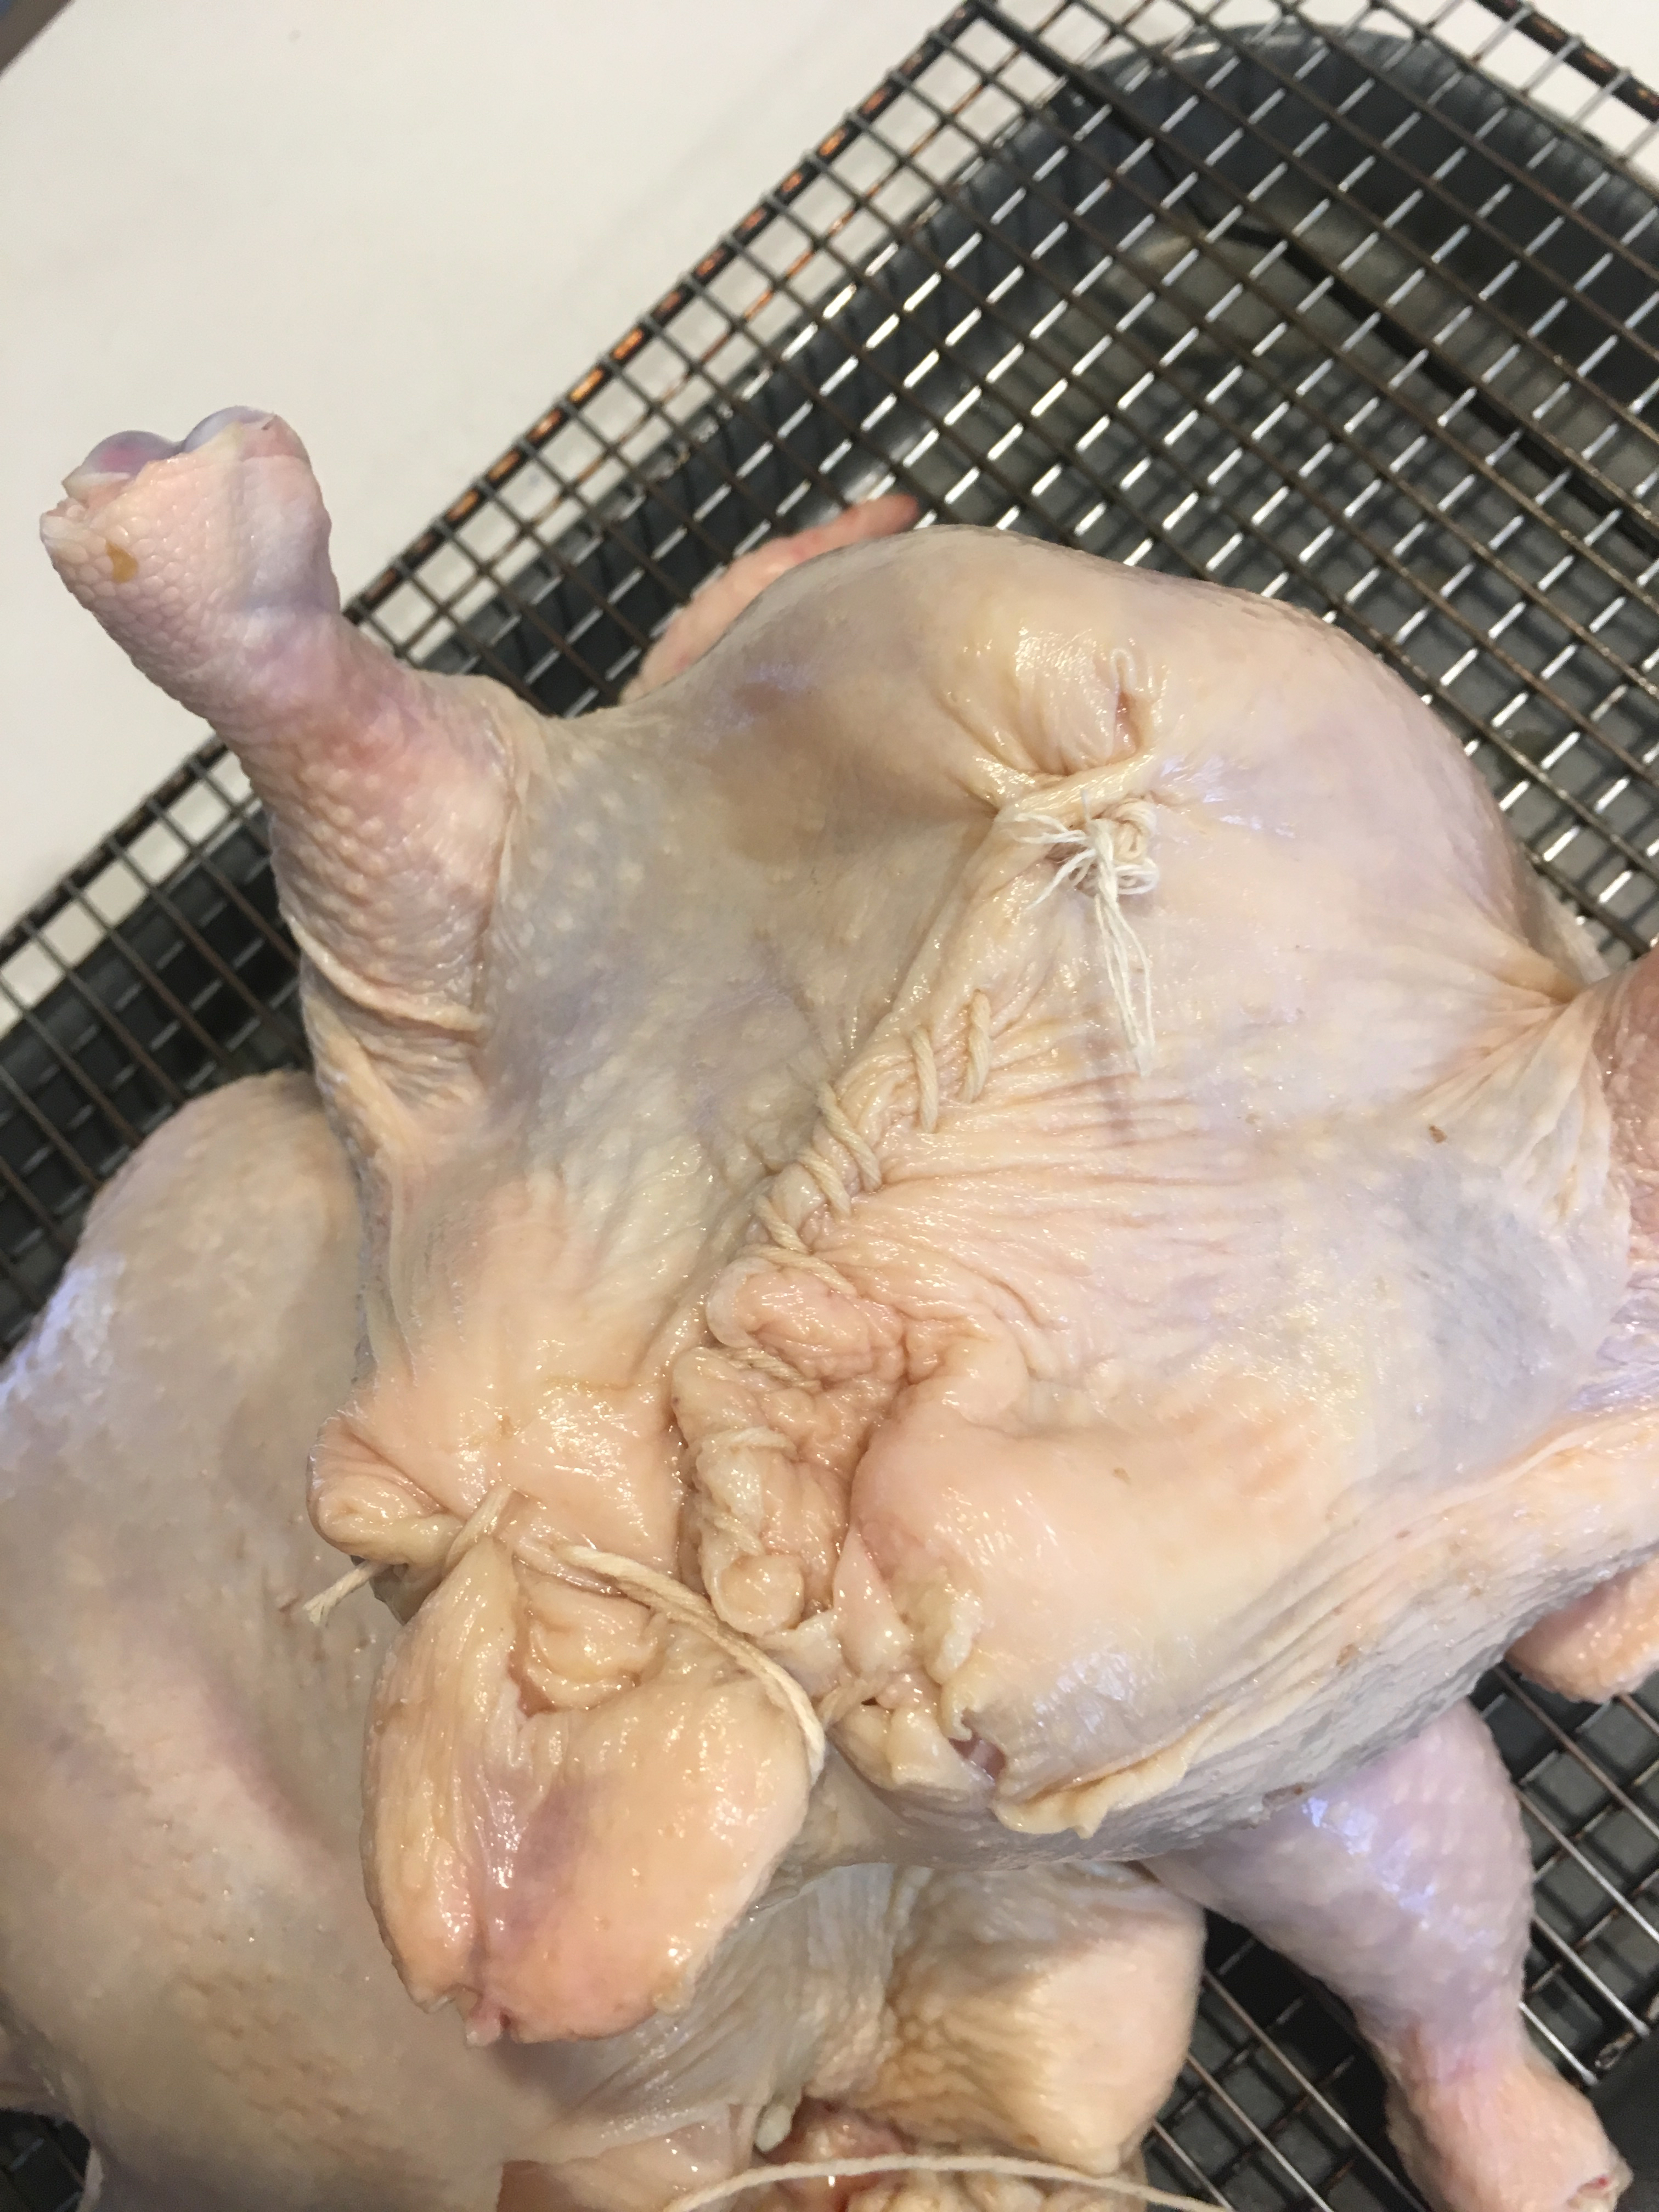
\includegraphics[width=0.25\textwidth]{\imageDir/\fileName/IMG_3217.jpg} &
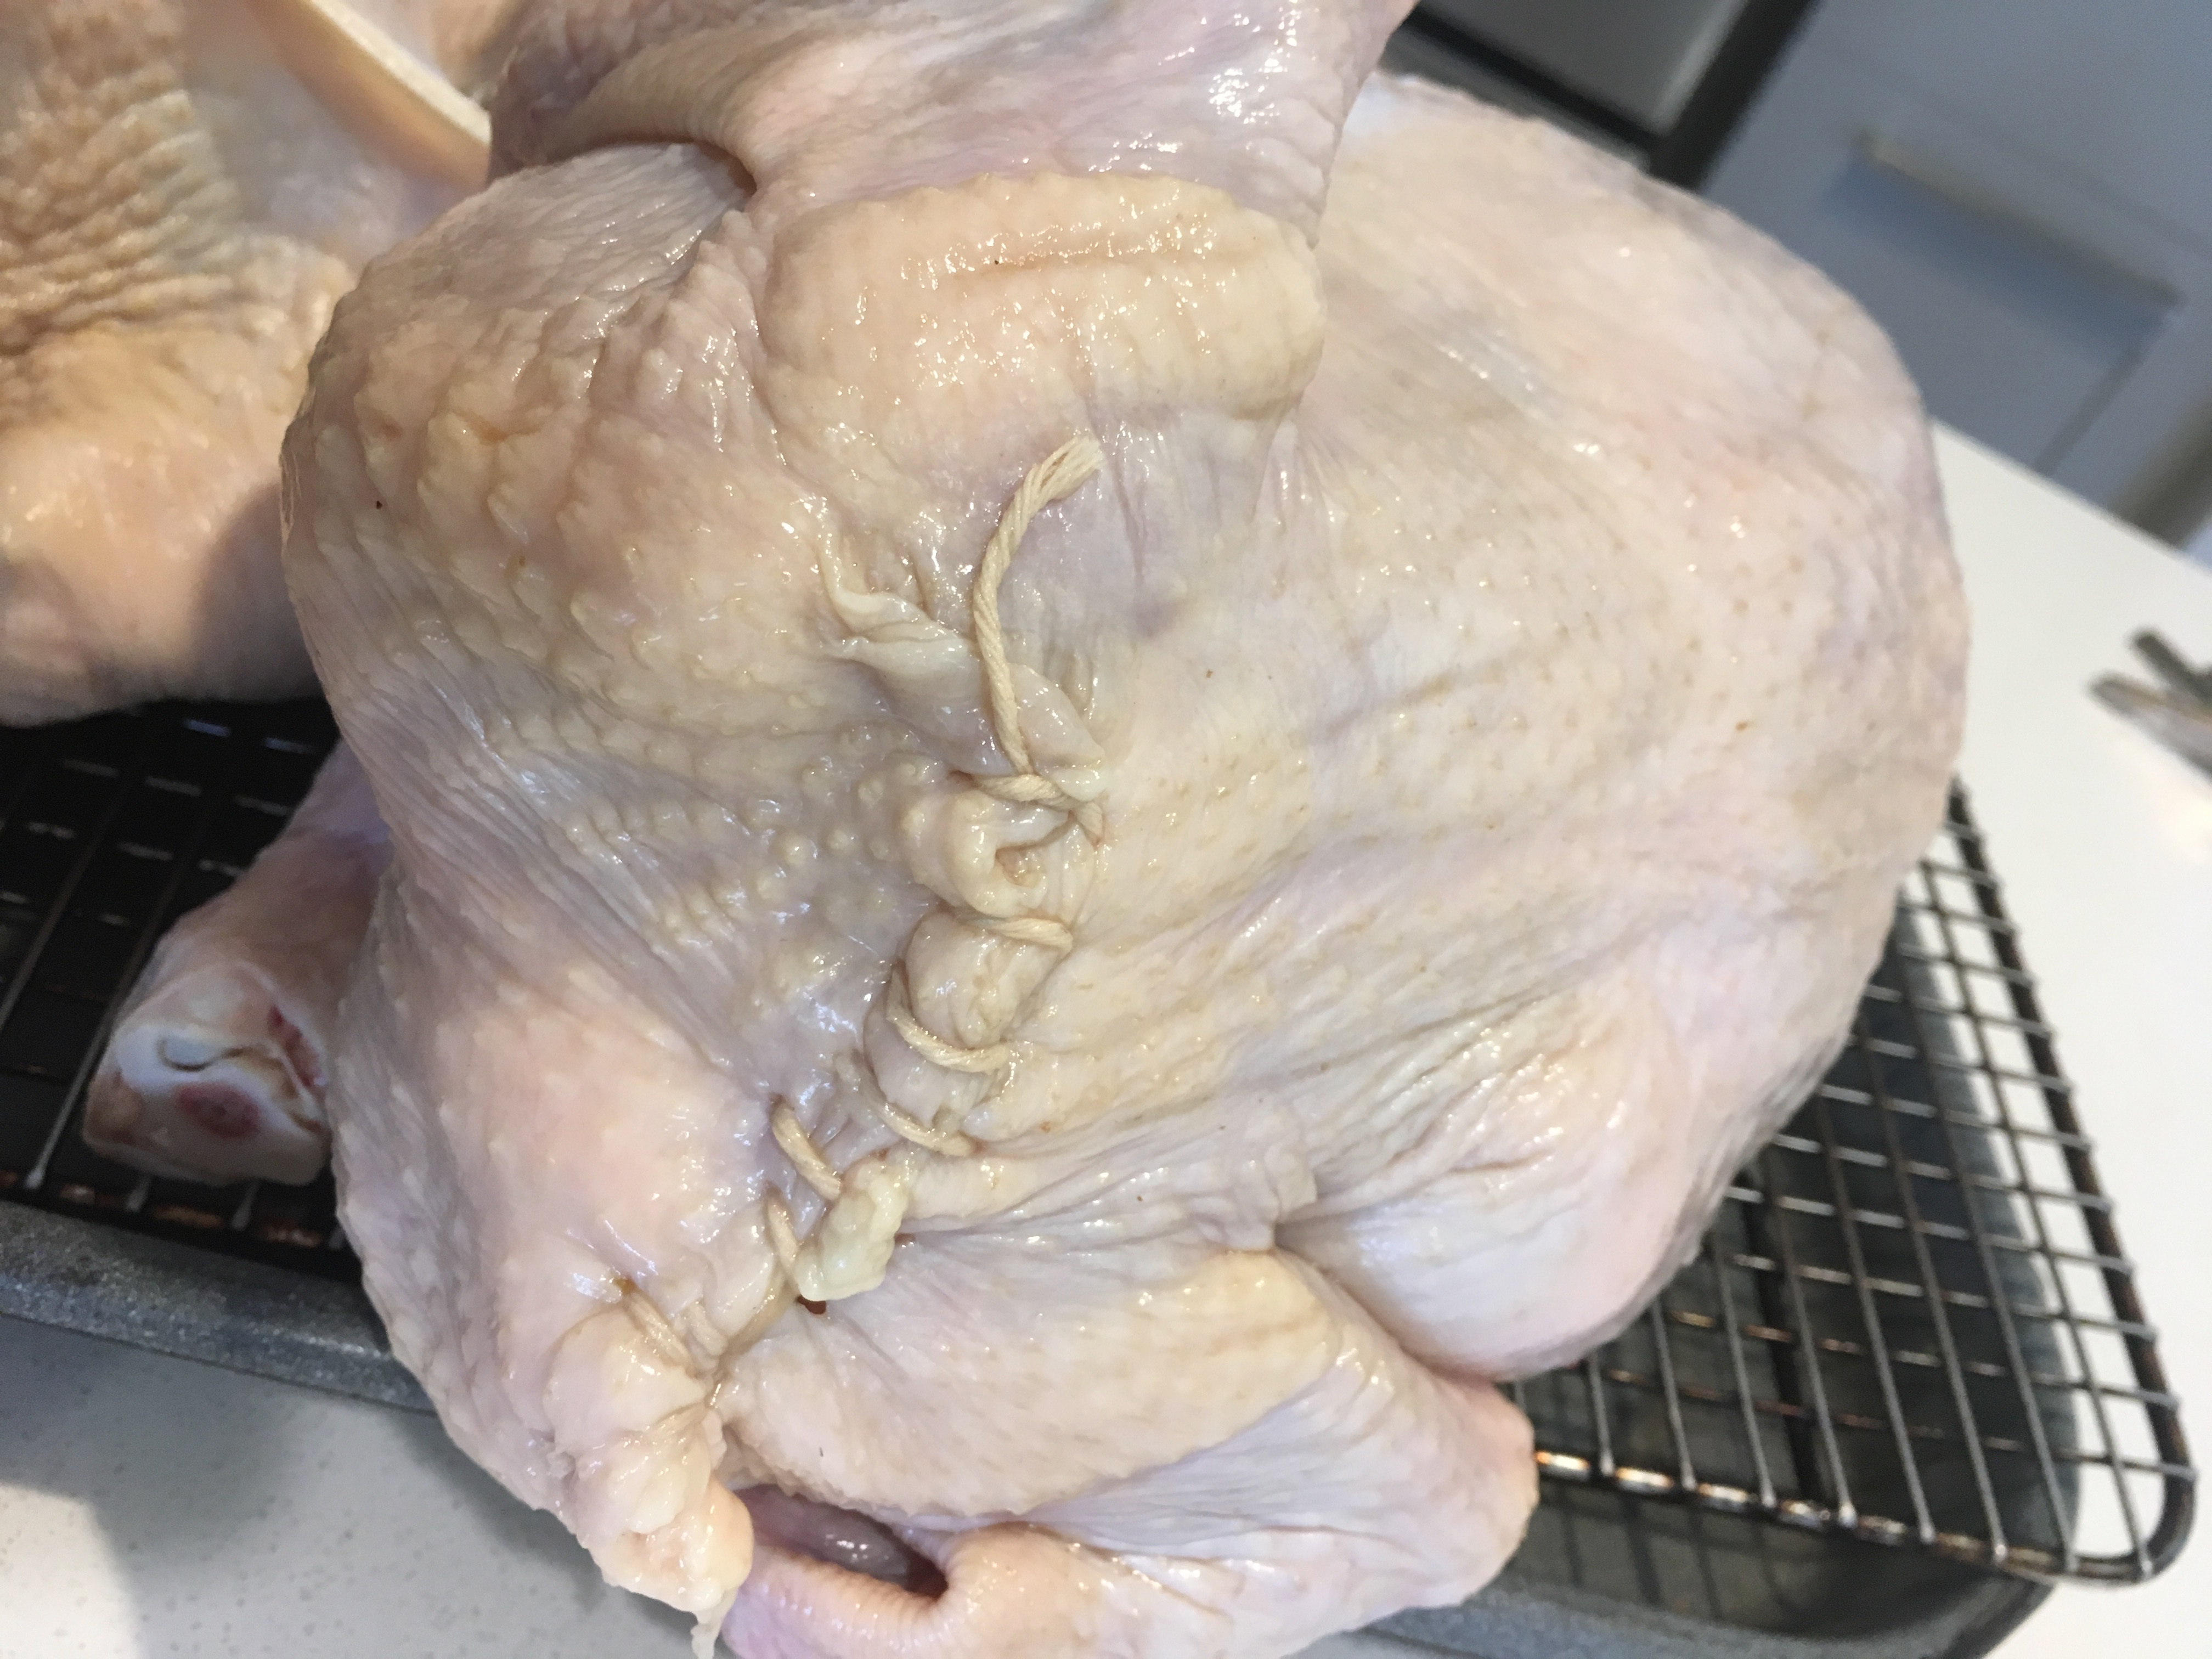
\includegraphics[width=0.25\textwidth]{\imageDir/\fileName/IMG_3218.jpg} &
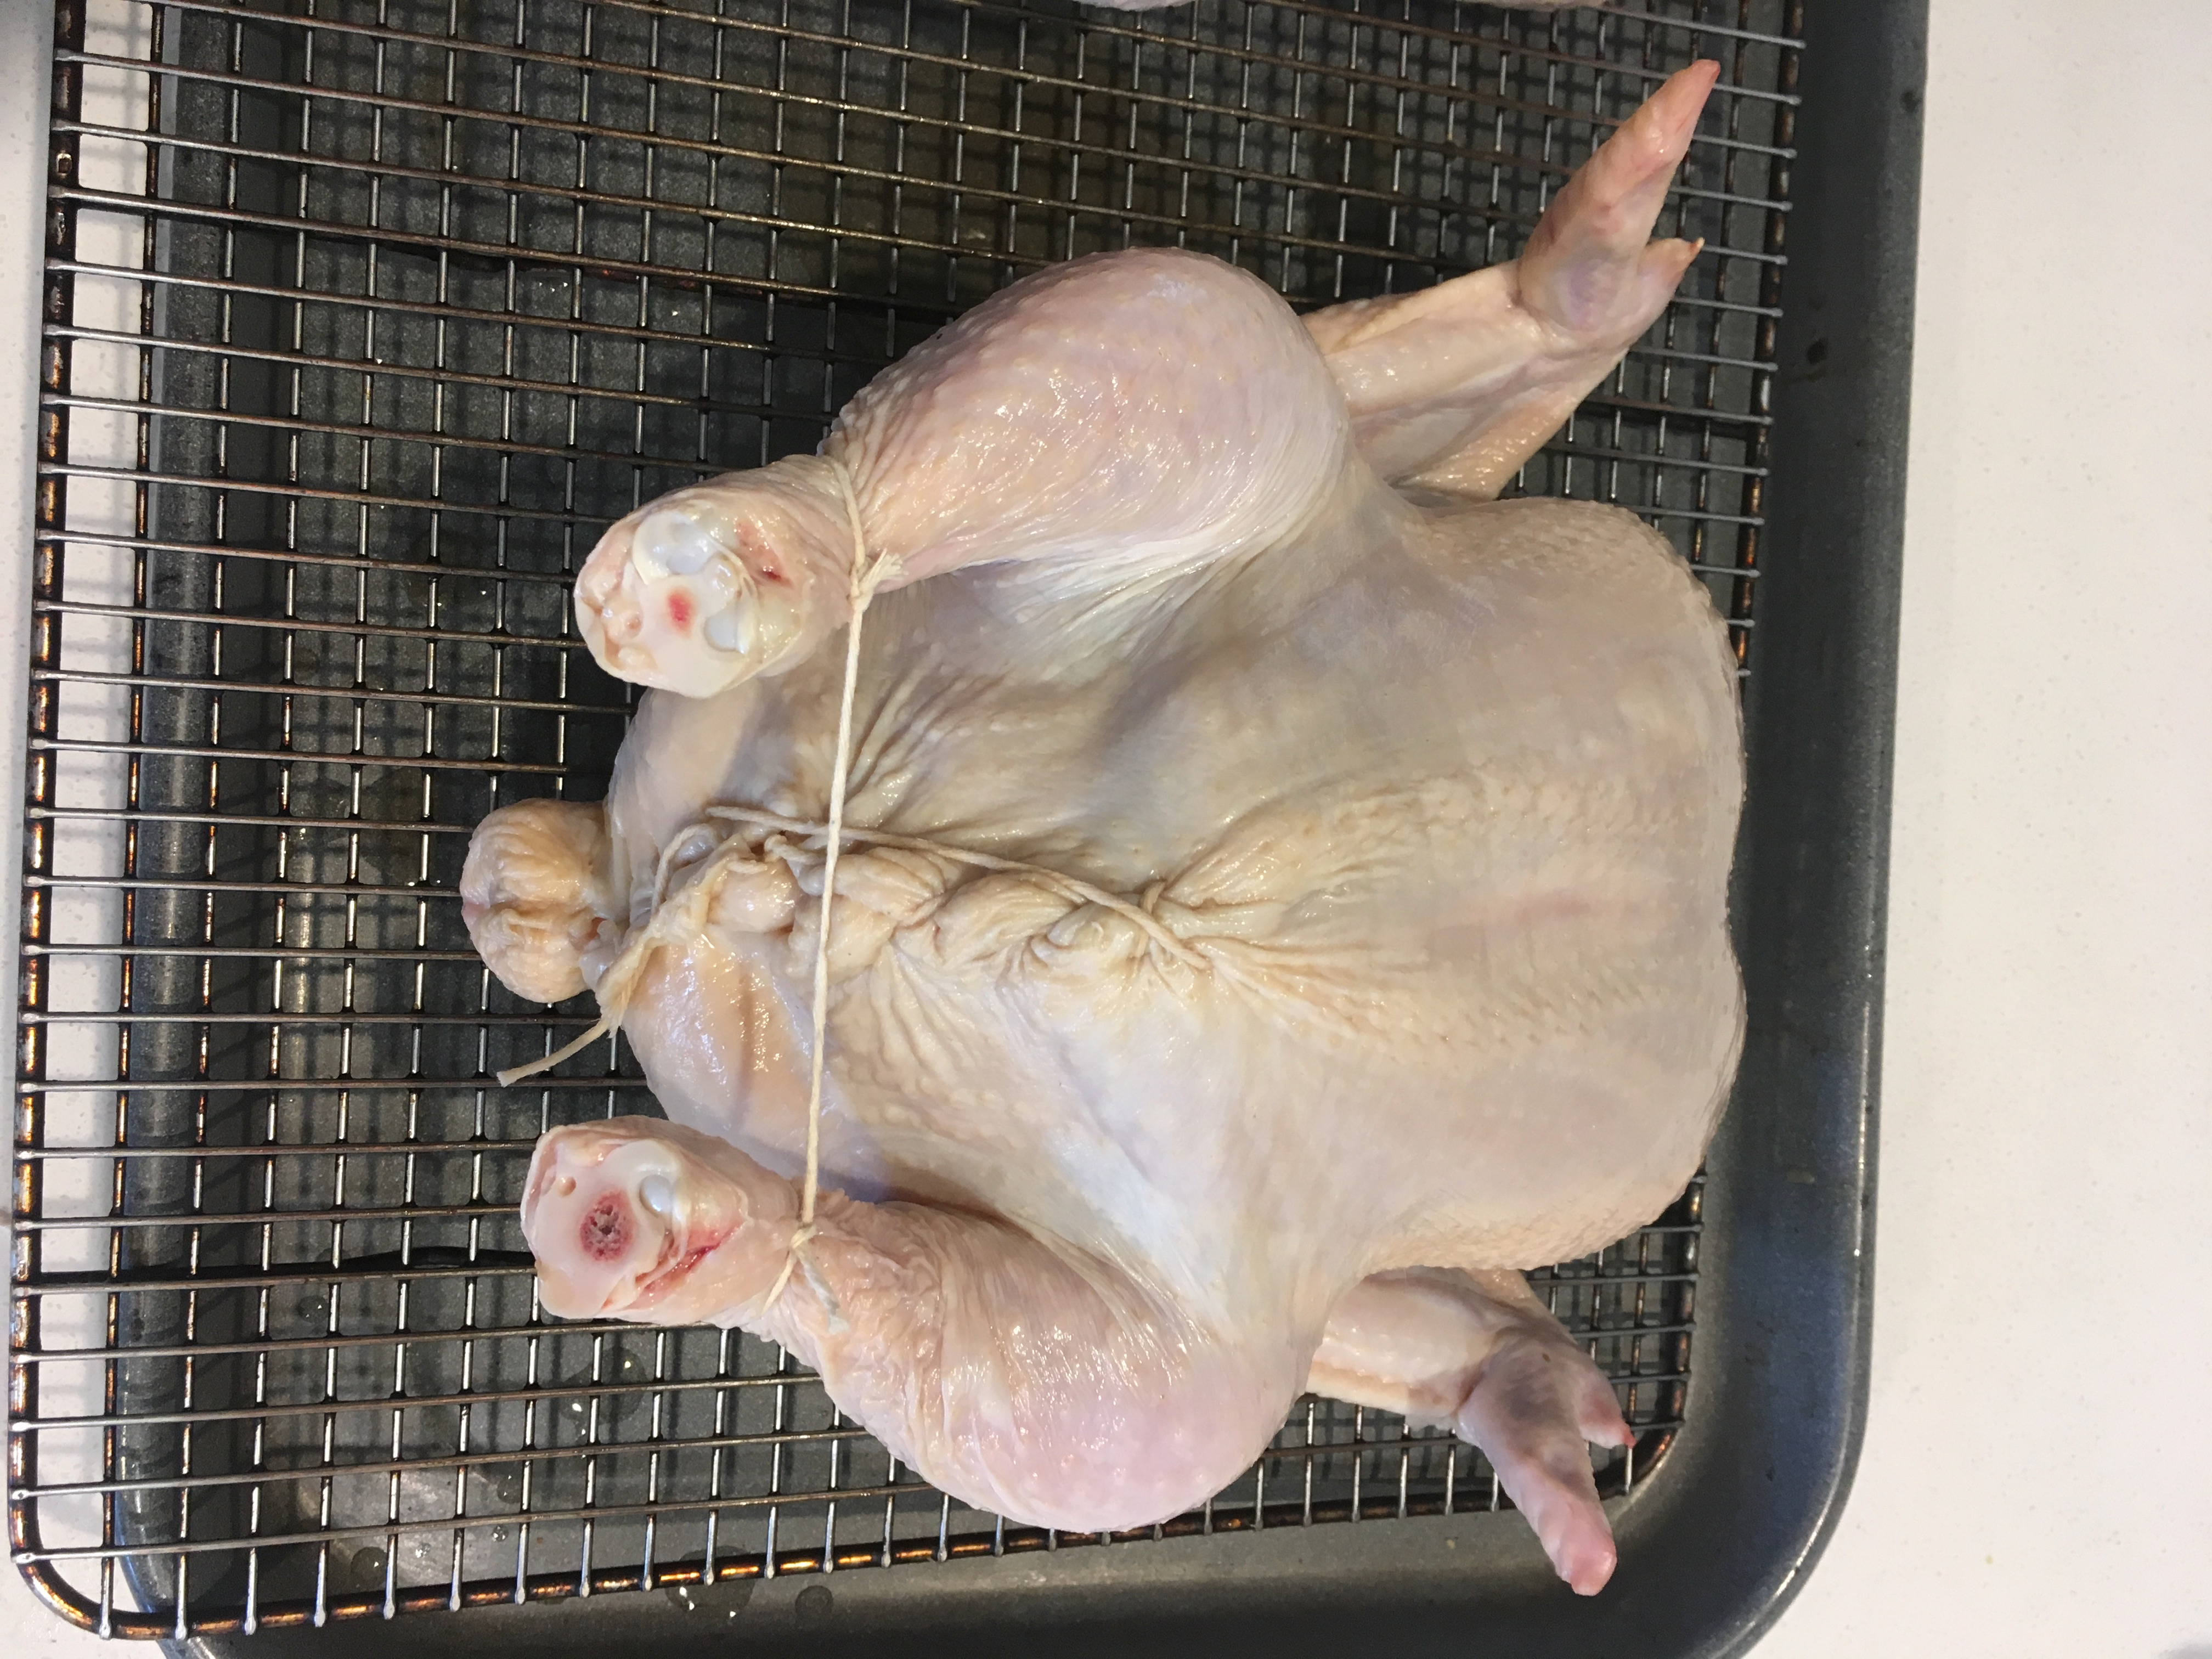
\includegraphics[width=0.25\textwidth]{\imageDir/\fileName/IMG_3219.jpg} \\
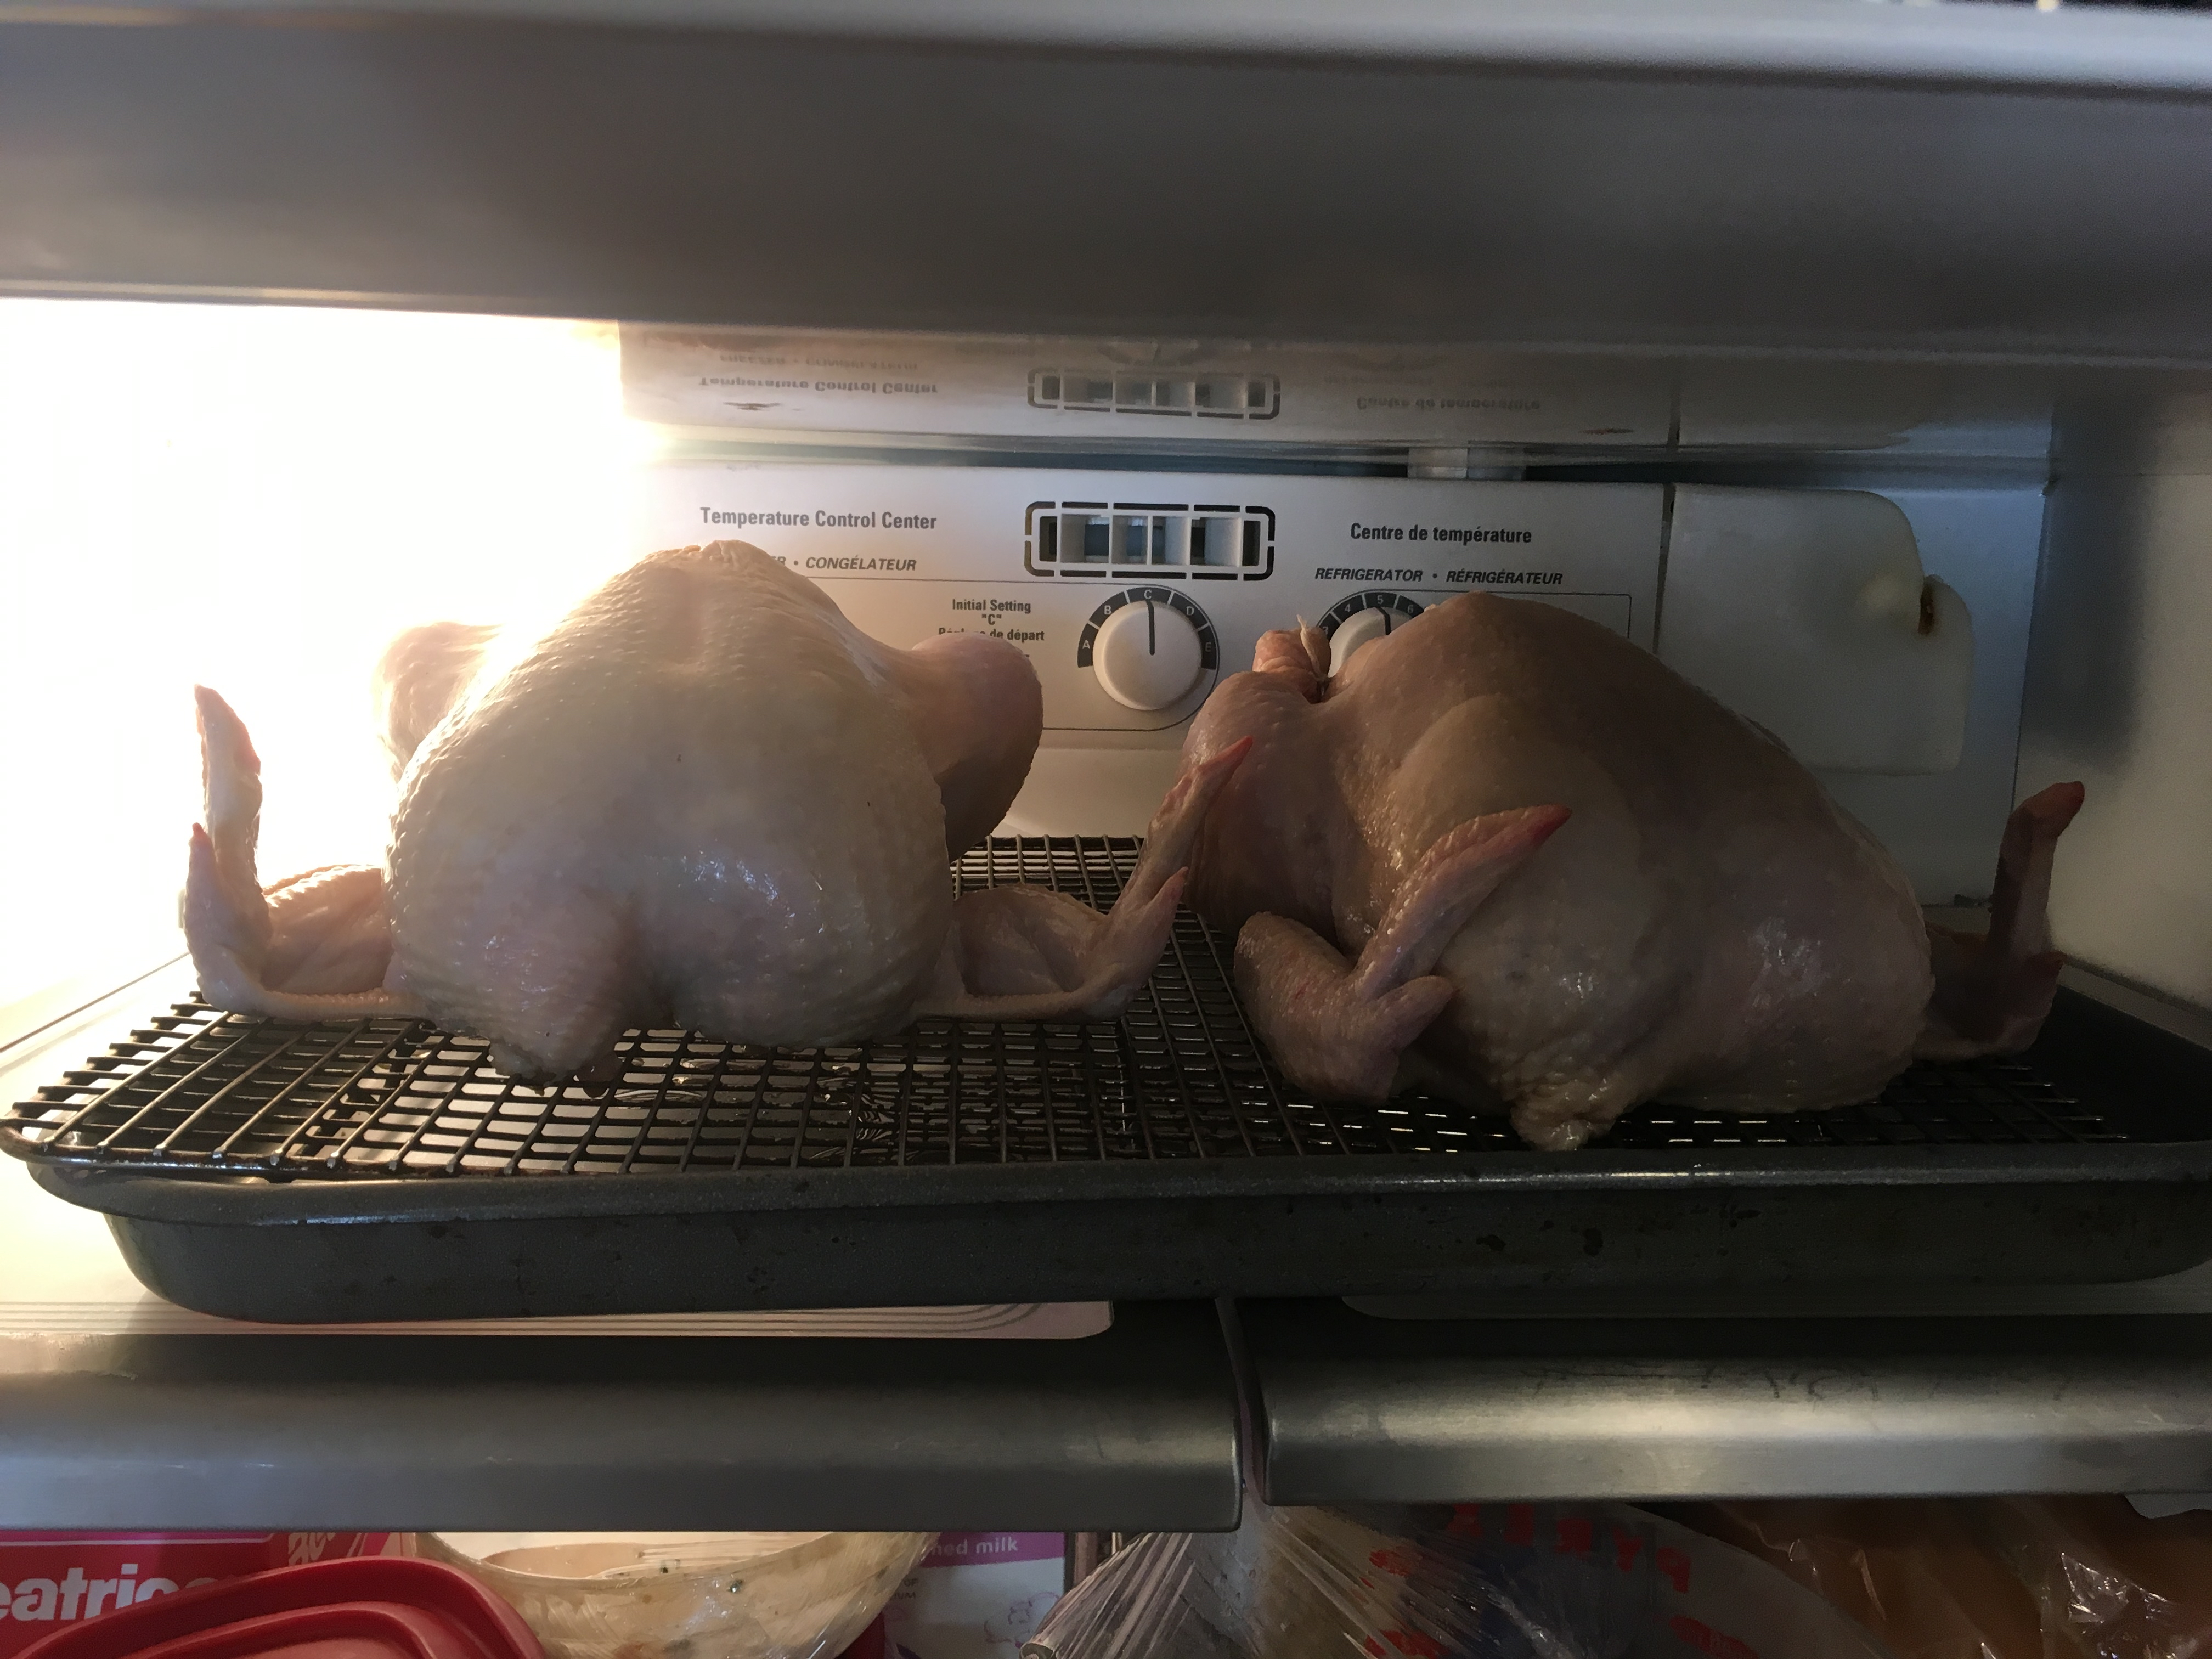
\includegraphics[width=0.25\textwidth]{\imageDir/\fileName/IMG_3220.jpg} &
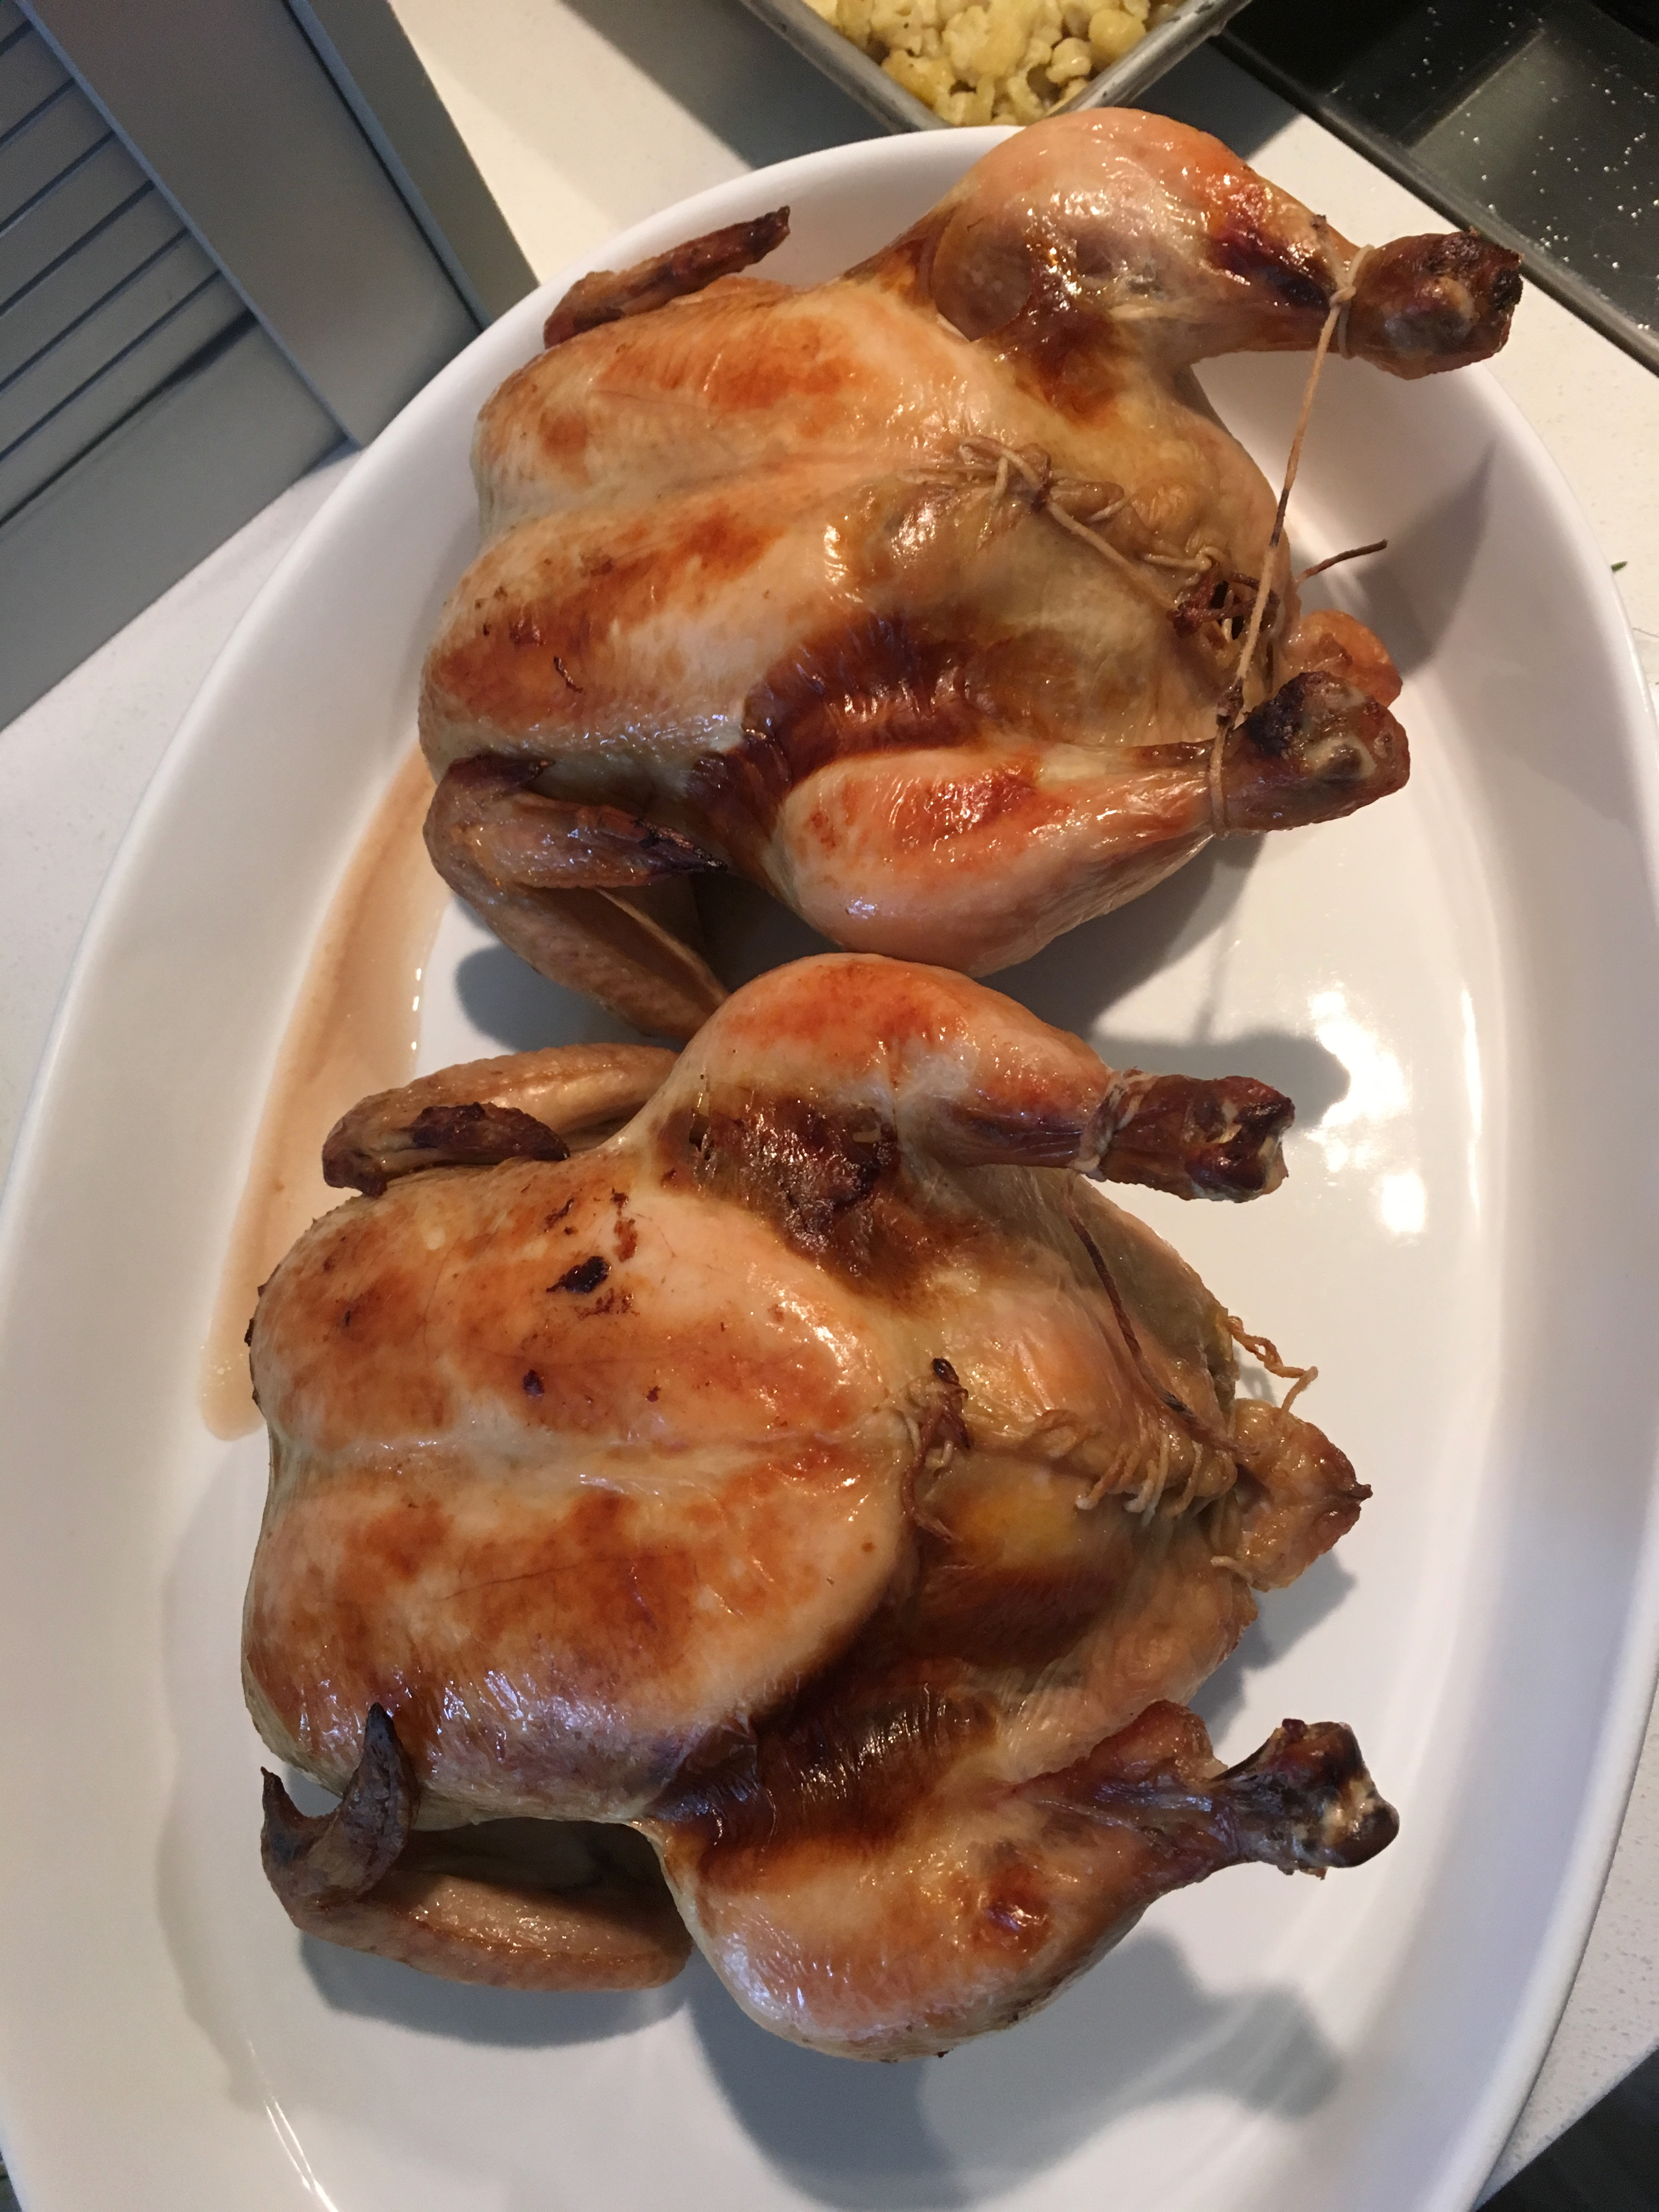
\includegraphics[width=0.25\textwidth]{\imageDir/\fileName/IMG_3228.jpg} \\
\end{tabular}
\end{table}

\end{document}



